\documentclass[wimgr]{xmgr}
%\documentclass[xodstep]{xmgr}

%\defaultfontfeatures{Scale=MatchLowercase}
%\setmainfont[Numbers=OldStyle,Ligatures=TeX]{Minion Pro}
%\setsansfont[Numbers=OldStyle,Ligatures=TeX]{Myriad Pro}
% for fontspec version < 2.0
\setmainfont[Numbers=OldStyle,Mapping=tex-text]{Minion Pro}
\setsansfont[Numbers=OldStyle,Mapping=tex-text]{Myriad Pro}
%\setmonofont[Scale=0.75]{Monaco}

% Opcjonalnie identyfikator dokumentu 
% drukowany tylko z włączoną opcją 'brudnopis':
\wersja   {}

\author   {Dorian Sawa}
\nralbumu {186\,445}
\email    {dsawa@sigma.ug.edu.pl}

\title    {System weryfikacji jakości kodu \newline w języku Scala}
\date     {2014}
\miejsce  {Gdańsk}

\opiekun  {dr Wiesław Pawłowski}

\usepackage{xunicode}
\usepackage{multirow}
\usepackage{booktabs}
\newcommand{\tabitem}{~~\llap{\textbullet}~~}
\usepackage{float}
\usepackage{alltt}
\usepackage{hyperref}
\usepackage{minted}
	\renewcommand\listingscaption{Przykład}
	
\makeatletter
\minted@define@extra{label}
\makeatother
	
\fvset{
	fontsize=\small
}

% dodatkowe polecenia
%\renewcommand{\filename}[1]{\texttt{#1}}

\begin{document}

\begin{abstract}
Scala to język wspierający paradygmaty programowania obiektowego i funkcyjnego. Rosnąca w ostatnim czasie popularność Scali przyczyniła się do powstania wielu narzędzi pozwalających na testowanie programów napisanych właśnie w tym języku. Niniejsza praca zgłębia temat wspomnianych narzędzi oraz ich wykorzystania jako podstawy systemu pozwalającego na automatyzację kontroli jakości kodu.
\end{abstract}
\keywords{Scala, 
 Play Framework, 
 Simple Build Tool,
 ScalaTest, 
 ScalaCheck}

% tytuł i spis treści
\maketitle
%
% wstęp
\introduction Scala jest nowoczesnym językiem programowania działającym na wirtualnej maszynie Javy. Przez cały czas -- od chwili opublikowania jest językiem stale rozwijanym. Powstało wiele narzędzi i bibliotek wprowadzających do Scali ciekawe rozwiązania związane z testowaniem kodu, czy programowaniem współbieżnym. Współcześnie wiele szanowanych firm korzysta z systemów napisanych w tym języku. Napisane dla celów wewnętrznych, czy też komercyjnych spełniają swoje zadania z sukcesami. Wśród firm korzystających z technologii Scali znaleźć można między innymi LinkedIn, Twitter czy Intel. 

Scala jest językiem całkowicie zorientowanym obiektowo. Posiada również wszystkie elementy jakich można oczekiwać od języka funkcyjnego. Sprawnie łączy ze sobą te dwie techniki programowania. Ponadto, jest to język statycznie typowany, który zachęca do pisania czytelnego i zwięzłego kodu. Przy wielu zaletach jakie ze sobą niesie możliwość programowania w Scali, udział procentowy tego języka na tle konkurencji jest wciąż stosukowo nieduży. Oczywiście proporcjonalnie do takiego rozkładu wygląda również sytuacja programistów Scali na rynku pracy. Jednym z impulsów do zmiany tego faktu mogłaby być specjalna platforma pozwalająca przyspieszyć proces nauki Scali. Na tym zagadnieniu skupia się niniejsza praca.

Zaprojektowany i opisywany system powstał na bazie nowoczesnych technologii oraz najważniejszych narzędzi do tworzenia testów jednostkowych. Składa się~z~dwóch aplikacji internetowych powstałych przy pomocy \emph{Play Framework}. Narzędzie to pozwala na szybkie napisanie aplikacji internetowej zarówno w Scali jak~i~w Javie. Społeczność zgromadzona wokół tych dwóch języków doprowadziła do powstania ogromnej liczby bibliotek. Z powodzeniem mogą być one używane~w~aplikacji utworzonej przy użyciu Play Framework. Cały system jest dostosowany do pracy w architekturze rozproszonej. 

Pośród bibliotek związanych z testowaniem kodu na szczególną uwagę zasługują ScalaTest i ScalaCheck. Pierwsza z nich to biblioteka do przeprowadzania testów jednostkowych. Umożliwia ona między innymi pisanie testów w wielu różnych stylach. Decyzja o tym jak ostatecznie wyglądać będzie test zależy od preferencji użytkownika. ScalaCheck jest zaś instrumentem służącym do testowania funkcji, metod poprzez automatyczne wywoływanie ich z różnymi, losowo generowanymi, zestawami argumentów. Te dwa narzędzia stanowią esencję opisywanego systemu. Proces analizujący kod wykorzystuje bowiem mechanizm testów jednostkowych.  

Weryfikacja kodu użytkowników systemu jest bezpośrednio związana z \emph{Simple Build Tool} -- SBT. Narzędzie to pozwala stworzyć szkielet projektu dla Scali. System traktuje projekt SBT jako zadanie przygotowane dla grupy osób. Wykonując serię testów jednostkowych dla danego projektu jest w stanie wystawić ocenę danemu użytkownikowi. Wszystkie informacje zgromadzone w procesie weryfikacji przechowywane są w nierelacyjnej bazie danych -- \emph{MongoDB}. Posiada ona wbudowany mechanizm do przechowywania plików. Dzięki temu, możliwe jest komfortowe zarządzanie projektami przesyłanymi do systemu.

Interfejs użytkownika powstał przy pomocy \emph{AngularJS}. Dzieło inżynierów firmy Google, które w przyjemny dla programisty sposób potrafi stworzyć dynamiczne strony HTML. Poszczególne elementy strony mogą być powiązane dwukierunkowo~z~modelami aplikacji. Efekty akcji użytkownika mających wpływ na stan modeli, automatycznie jest prezentowany w odpowienich widokach. AngularJS pozwala również na wzbogacanie składni HTML o nowe atrybuty i elementy. Zostają one zinterpretowane przez niego w sposób określony przez programistę.

Dla innych języków programowania już funkcjonują pewne mechanizmy edukacyjne. Scala zasługuje również na to, aby więcej osób mogło ją poznać. Kombinacja języka funkcyjnego i obiektowego oraz wiele innych aspektów jakie ze sobą niesie ten język są cechami, z którymi każdy przyszły, a nawet już doświadczony programista powinien się zapoznać. 

Wszystkie wspomniane wcześniej narzędzia miały wpływ na ostateczny kształt opisywanego systemu. W niniejszej pracy zostaną one szerzej przedstawione wraz z działaniem systemu weryfikacji jakości kodu Scala.

\chapter{Idea systemu}

Wykonując odpowiednie zapytanie przy użyciu narzędzia \textit{Google BigQuery} oraz danych z \textit{Github Archive} można w prosty sposób sprawdzić popularność języków programowania na platformie \textit{GitHub}. Ilość repozytoriów dla poszczególnych języków w roku 2013  przedstawia rysunek \ref{RYS.1}. 

\begin{figure}[!tbh]
\centering 
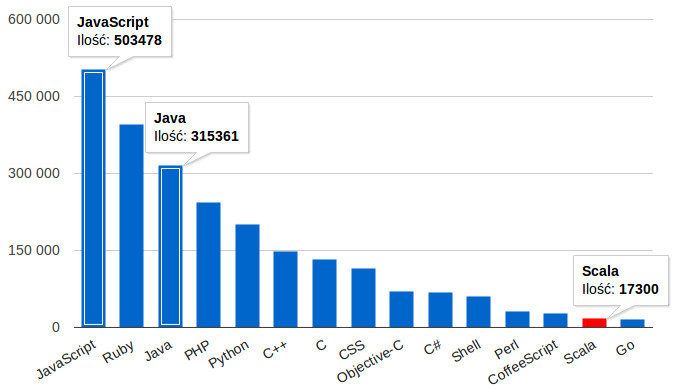
\includegraphics[width=.95\hsize]{fig/top_github_languages_2013}
\caption{Ilość repozytoriów dla poszczegónych języków na platformie GitHub~w~roku 2013 \label{RYS.1}}
\source{GitHub Archive (www.githubarchive.org)}
\end{figure}

Powyższy wykres przedstawia pierwszych 15 języków, wśród których Scala uplasowała się na miejscu 14. Różnica w liczbie repozytoriów między Scalą, a Javą będącą na trzecim miejscu jest znaczna. Nie ma wątpliwości, że Java swoją wysoką pozycje zawdzięcza wieloletniej obecności na rynku, a także wkładowi jaki do świata technologii informacyjnych wniosła maszyna wirtualna JVM. Na popularność JavaScript'u, czy Ruby'ego częściowo miało wpływ pojawienie się w ostatniej dekadzie narzędzi takich jak \textit{Ruby on Rails}, \textit{node.js}, \textit{AngularJS} i wielu innych. 

Jednak jak pokazuje przykład Ruby'ego i JavaScriptu, jednym z elementów wpływających na popularność jest aktywne środowisko programistów zgromadzonych wokół danego języka. Niejednokrotnie, taka grupa osób przekonana o zaletach swojego ulubionego języka jest w stanie wytworzyć alternatywne sposoby jego promocji. Potwierdzeniem tego może być zespół programistów zgromadzonych wokół platformy \textit{CodeSchool}\footnote{\url{www.codeschool.com}}. Opracowali oni szereg prostych kursów związanych głównie z JavaScript'em i Ruby'm, w trakcie których uczestnik rozwiązuje proste zadania programistyczne. 

Żadne z obecnych rozwiązań -- szczególnie dla Scali -- nie posiada jednak możliwości tworzenia własnych zadań dla zamkniętych grup uczestników. Wierzę, że system, który daje sposobność definiowania własnych kursów dla języka Scala może znacząco zwiększyć jego popularność. Użycie takiego systemu w szkołach~i~uczelniach mogłaby przynieść również inne korzyści, jak na przykład wzrost zainteresowania programowaniem, czy podniesienie umiejętności przyszłych programistów przy jednoczesnym zmniejszeniu nakładu pracy prowadzących zajęcia.

\section{Język Scala}

Pomysłodawcą i głównym twórcą Scali jest niemiecki profesor Martin Odersky. Nazwa języka ma na celu sugerować, że jest on skalowalny\footnote{ang: Scalable language}. Scala rośnie wraz~z~potrzebami jej użytkowników. Cały czas powstają kolejne narzędzia i biblioteki mające uprościć pracę z nią, czy też dodać do niej nowe mechanizmy. 

Jedną z ciekawostek wprawdzonych przez Scalę jest środowisko o nazwie REPL\footnote{ang: Read-Evaluate-Print Loop}. Jest to interfejs do kompilatora, który można traktować jak ,,interpreter''. REPL potrafi między innymi podpowiedzieć ścieżki do pakietów i klas, czy możliwe do wywołania metody na danych bytach po wciśnięciu klawisza tabulacji. Jest to doskonałe narzędzie do sprawdzania małych fragmentów kodu.

Scala łączy ze sobą paradygmat programowania obiektowego oraz funkcyjnego. Umożliwia wykorzystanie najlepszych cech tych dwóch podejść w projektowaniu nowych systemów. Sprawdzi się zatem doskonale zarówno podczas pisania małych jak i dużych projektów.

W przypadku tych pierwszych, programowanie funkcyjne w większości jest dobrym wyborem. Mogą one posiadać stały zestaw komponentów, na przykład w postaci klas. Wraz z ewolucją kodu, dodawane są głównie nowe operacje na istniejących bytach. Dokonuje się tego poprzez dodawanie nowych funkcji, które wykonują obliczenia opierając się na istniejących typach danych. 

Programowanie obiektowe jest dobrym wyborem kiedy dysponujemy stałym zestawem operacji na komponentach programu, a w czasie ewolucji kodu dodawane są nowe byty jak klasy. Gdy istnieje, więc potrzeba zaimplementowania dużego systemu, który będzie wymagać rozwijania i dostosowywania do nowych potrzeb, paradygmat programowania obiektowego sprawdzi się lepiej.

\subsection{Aspekt obiektowy}

Scala jest zorientowana obiektowo. Inaczej jednak, niż w wielu językach obiektowych, nie posiadamy tutaj wartości, które nie są obiektami jak np. typy prymitywne w Javie. Każda wartość jest obiektem, a każda operacja jest wywołaniem metody. 

Ponadto zezwala ona na zdefiniowanie metod o nazwie przypominającej operator. Przykładem może być metoda \texttt{:::} konkatenująca listy, czy metoda \texttt{!} w klasie \texttt{Actor}. Tworzenie nowych obiektów w Scali jest również bardzo elastyczne. Komponent zwany cechą (ang. trait) jest czymś, czym dla Javy są interfejsy. Jednak~w~porównaniu do interfejsów, cechy mogą zawierać implementacje pól oraz metod. 

Dzięki cechom, Scala idzie także o krok dalej w kwestii kreowania obiektów. Dobrym przykładem tego może być wielokrotne dziedziczenie, które można osiągnąć w poniższy sposób.

\inputminted[fontsize=\small]{scala}{code/multipleInheritance.scala}

Należy w uzupełnieniu do powyższego przykładu wspomnieć jak Scala interpretuje konstrukcję \texttt{super}. Otóż będzie ona wywołana zawsze~w~tym miejscu,~w~którym się pojawia. Odpowiada za to proces linearyzacji. Podczas tworzenia instancji danej klasy, Scala układa wszystkie klasy i cechy, po których ta klasa dziedziczy w liniowej kolejności. Dowodem niech będzie wywołanie metody \texttt{get} dla wcześniej pokazanego kodu w interpreterze Scali.

\begin{minted}[fontsize=\small]{scala}
scala> new MyNumber(5).get
res0: Int = 9
\end{minted}

Liczba 5 została tutaj najpierw zmniejszona o 1, następnie pomnożona przez 2 i ostatecznie dopiero na końcu powiększona o 1. Zmieniając jednak kolejność cech wmieszanych w klasę \texttt{MyNumber} osiągniemy inny wynik.

\begin{minted}[fontsize=\small]{scala}
scala> class MyNumber(number: Int) extends Number(number: Int) 
         with Incrementing with Doubling with Decrementing
defined class MyNumber

scala> new MyNumber(5).get
res1: Int = 11
\end{minted}

Liczba 5 została tutaj najpierw zwiększona o 1, w następnym kroku pomnożona przez 2, by wynik tego działania pomniejszyć o 1. Metoda \texttt{get} zwraca w tym przypadku 11, wykonując działania w odwrotnej kolejności niż przedtem.

Warto wspomnieć również o klasach poprzedzonych modyfikatorem \texttt{case}. Kompilator Scali dodaje kilka udogodnień dla takich bytów. 

Pierwszym z nich jest dodanie metody \texttt{apply} do tak zwanego ,,obiektu stowarzyszonego'' (ang: companion object) z daną klasą. Jest to specjalny obiekt o nazwie identycznej jak sama klasa. W praktyce oznacza to, że tworząc nowy obiekt takiego typu nie jest obowiązkowym podawanie instrukcji \texttt{new}. 

\begin{minted}[fontsize=\small]{scala}
scala> case class MyNumber(number: Int)
defined class MyNumber

scala> val mn = MyNumber(5)
mn: MyNumber = MyNumber(5)
\end{minted}

Drugim ułatwieniem jest fakt, że wszystkie argumenty automatycznie stają się polami danej klasy. Dla porównania, w klasach bez modyfikatora \texttt{case} nie można się odwołać do nich z zewnątrz, a żeby parametr był rozpatrywany jako pole wymaganym jest podanie prefiksu \texttt{val}.

\begin{minted}[fontsize=\small]{scala}
scala> class Cat(name: String)
defined class Cat

scala> case class Dog(name: String)
defined class Dog

scala> new Cat("Nazir").name
<console>:9: error: value name is not a member of Cat
              new Cat("Nazir").name
scala> Dog("Luna").name
res7: String = Luna           
\end{minted}

Trzecim udogodnieniem są implementacje metod \texttt{toString}, \texttt{hashCode} oraz \texttt{equals}. Pierwsza z nich zwróci ciąg znaków w postaci nazwy klasy wraz z aktualnymi wartościami pól. Wynikiem wywołania metody \texttt{hashCode} będzie oczywiście unikalny kod mieszający obiektu. Ostatnia z wymienionych, potrafi porównać całe drzewo klas i w sposób rekursywny wszystkie argumenty obiektów. Ponieważ~w~Scali operator \texttt{==} zawsze odwołuje się do metody \texttt{equals} to tego typu klasy automatycznie porównywane są w sposób strukturalny.    

Komponentom z modyfikatorem \texttt{case} kompilator dodaje jeszcze jedną wygodną metodę -- \texttt{copy}. Zwraca ona kopię obiektu w postaci nowej instancji klasy, gdzie różne są wartości niektórych pól. Korzysta ona z parametrów opisanych nazwami. Gdy nie zostaje podana nazwa danego pola to zwracana jest stara, nie zmodyfikowana wartość. 

\begin{minted}[fontsize=\small]{scala}
scala> val d = Dog("Luna")
d: Dog = Dog(Luna)

scala> d.copy(name = "Azor")
res1: Dog = Dog(Azor)
\end{minted}

Jedynym kosztem użycia modyfikatora \texttt{case} przed definicją klasy jest fakt, że obiekty staną się nieco większe. Dzieje się tak z powodu dodatkowych metod. Największą zaletą jednak jest możliwość użycia takich klas w mechanizmie dopasowywania wzorca opisanego w późniejszej części tego rozdziału.

\subsection{Aspekt funkcyjny}

Jak wyjaśnia Martin Odersky, ,,programowanie funkcyjne w głównej mierze opiera się na dwóch założeniach'' \cite[s.57]{Odersky:2010:PIS}. Wskazane jest, aby funkcje były wartościami podstawowymi, a operacje wykonywane~w~czasie działania programu powinny zwracać wartości do nowych zmiennych niż modyfikować obecne. Obie te koncepcje są oczywiście obecne w Scali, w której funkcje są specjalnymi obiektami. 

Możemy przekazywać funkcję jako argument do innej funkcji, po to aby~w~odpowiedzi otrzymać jeszcze inną funkcję. Możliwe jest także definiowanie funkcji wewnątrz innych funkcji. Funkcje mogą posiadać nazwę lub być też anonimowe. Żadna z wymienionych opcji nie jest możliwa chociażby w Javie, aż do wersji 8, która to dopiero pozwala na użycie funkcji anonimowych. Wszystkie te warianty mają bezpośredni wpływ na skalowalność programów.

Inspiracja do poniższego przykładu pochodzi z książki ,,Scala by Example'' profesora Martina Oderskiego \cite[s. 22]{Odersky:2014:SBE}. Korzystając ze środowiska REPL pokazuje on~w~prosty sposób jak może wyglądać praca z funkcjami w Scali. Zdefiniowane zostały dwie funkcje -- \texttt{sum} oraz \texttt{sumSquares}.

\begin{minted}[fontsize=\small]{scala}
scala> def sum(f: Int => Int, a: Int, b: Int): Int = f(a) + f(b)
sum: (f: Int => Int, a: Int, b: Int)Int

scala> def sumSquares(a: Int, b: Int): Int = sum((x: Int) => x * x, a, b)
sumSquares: (a: Int, b: Int)Int

scala> sumSquares(3, 4)
res0: Int = 25
\end{minted}

Pierwszym parametrem \texttt{sum} jest funkcja (f), która za argumenty przyjmuje liczby całkowite. Zobligowana jest także do zwrócenia wartości tego typu. W ciele funkcji \texttt{sum} widać, że na pozostałych dwóch argumentach (a i b) wywołana zostaje funkcja \texttt{f}. Dodane do siebie zostają bowiem wartości \texttt{f(a)} i \texttt{f(b)}. Zdefiniowano więc funkcję posiadającą w liście argumentów inną funkcję. W ciele funkcji \texttt{sumSquares}, \texttt{sum} zostaje wywołana poprzez podanie jako pierwszego argumentu funkcji anonimowej.

Autorzy ,,Programming in Scala'' posłużyli się doskonałym przykładem wyjaśniającym drugie założenie. \cite[s.57]{Odersky:2010:PIS} Otóż należy rozpatrzeć implementacje ciągu znaków w języku Ruby i Java. W Ruby'm, ciag znaków jest niczym innym jak tablicą znaków. Możemy zatem każdy znak w danym ciągu podmieniać wewnątrz tego samego obiektu. W Javie, typ \texttt{String} jest ciągiem znaków w sensie matematycznym. Aby wykonać podobną operację konieczne jest wywołanie metody \texttt{replace}, która zwraca zupełnie nowy obiekt.

Prawdziwy język funkcyjny wymusza na programiście, aby ten korzystał z niezmiennych danych. Scala daje możliwość wyboru, ale jednocześnie zachęca do unikania imperatywnych konstrukcji. Pracując z funkcyjnym językiem programowania nie unikniemy także niezmiennych struktur danych. Scala posiada również własny zestaw niezmiennych typów jak na przykład listy, czy zbiory. Idea wykonywania operacji na nich jest zbliżona do koncepcji niezmiennych wartości.

\begin{minted}[fontsize=\small]{scala}
scala> val list = List(1,2,3)
list: List[Int] = List(1, 2, 3)

scala> list :+ 4
res0: List[Int] = List(1, 2, 3, 4)
\end{minted}

Dla przykładowej trzyelementowej listy liczb całkowitych, wykonując operację dodawania nowego elementu do niej w wyniku zwrócony zostaje nowy obiekt reprezentujący listę czteroelementową. W imperatywnym języku programowania, taka operacja zmodyfikowałaby wcześniej utworzony obiekt. 

\subsection{Pozostałe cechy}

Oprócz łączenia technik programowania obiektowego i funkcyjnego, Scalę definują cechy takie jak kompatybilność z JVM, zwięzłość, wysoki poziom abstrakcji~i~statyczne typowanie. 

\subsubsection{Kompatybilność}

Wydajność programów napisanych w Scali jest porównywalna z odpowiednikami napisanymi w Javie. Programy te bowiem kompilują się do pseudokodu wirtualnej maszyny Javy. Ponadto są w stanie bez przeszkód wywoływać metody klas Javy, korzystać z ich pól, a nawet przystosowywać własne komponenty poprzez dziedziczenie klas Javy, czy implementację interfejsów. Każdy z tych wariantów jest wykonywany przez programistę w sposób naturalny, gdyż nie wymaga to użycia żadnej dodatkowej składni. Jak się okaże później, system będący głównym tematem pracy również korzysta z dobrodziejstw owej kompatybilności. Korzysta on z oficjalnego klienta dla systemu kolejkowania wiadomości \emph{RabbitMQ} dla języka Java.

Scala korzysta w pełni z typów Javy. Typ \texttt{Int} w Scali reprezentuje prymitywne liczby całkowite \texttt{int} z Javy. Podobnie ma się sytuacja z \texttt{Float}, \texttt{Double}, \texttt{Long}, czy \texttt{Boolean}. Ponadto typy zostają ,,opakowowane'' w taki sposób, aby wywołania metod związanych z nimi były bardziej przejrzyste. W efekcie tego, dla przykładu zamiast \texttt{Double.parseDouble("12.0")} wystarczy napisać \texttt{"12.0".toDouble}.

\subsubsection{Zwięzłość}

Scala zachęca do zwięzłego i czytelnego stylu programowania. Porównując kod Scali i Javy ze sobą, niejednokrotnie okazuje się, że kod Scali jest krótszy o ponad połowę. Pozwala to na tworzenie kodu bardziej zrozumiałego, łatwiejszego w utrzymaniu przy jednoczesnym zmniejszeniu wysiłku programisty. Wynika to głównie ze składni języka, gdzie między innymi średniki na końcu instrukcji są opcjonalne. Pisząc funkcję, w wielu miejscach można pominąć klamry otwierające i zamykajace dany blok kodu. Jednak najbardziej tą różnicę pokazuje porównanie tworzenia klas z konstruktorem.

\medskip 

\inputminted[fontsize=\small,label=Person.java,frame=single,framerule=0pt,framesep=2pt]{java}{code/person.java}

\inputminted[fontsize=\small,label=Person.scala,frame=single,framerule=0pt,framesep=2pt]{scala}{code/person.scala}

\subsubsection{Wysoki poziom}

Język wysokiego poziomu to taki, który pozwala człowiekowi szybko zrozumieć kod programu. Scala jest typem takiego języka. Programista może przy pomocy dostępnych mu komponentów takich jak cechy, czy literały funkcyjne w dużo lepszy sposób zarządzać poziomem skomplikowania kodu. Znów warto w tym momencie porównać ze sobą Javę i Scalę. Niech problemem do rozwiązania, będzie znalezienie wszystkich liczb parzystych z przedziału od 1 do 10. W Scali to zagadnienie można rozwiązać w jednej linijce.

\mint[fontsize=\small]{scala}/val evenNumbers = (1 to 10).toList.filter(_ % 2 == 0)/

Natomiast w Javie, ten sam problem wymaga od programisty odpowiednio więcej pracy.

\begin{minted}[fontsize=\small]{java}
List<Integer> numbers = Arrays.asList(1, 2, 3, 4, 5, 6, 7, 8, 9, 10);
List<Integer> evenNumbers = new ArrayList<Integer>();
for(Integer number: numbers){
    if(number % 2 == 0){
        evenNumbers.add(number);
    }
}
\end{minted}

W drugim rozwiązaniu potrzebne były dwie listy oraz pętla iterująca po wszystkich liczbach z danego zakresu. W Scali wystarczy użyć odpowiedniej metody (\texttt{filter}), która jako argument przyjmuje predykat \texttt{\_ \% 2 == 0 }, będący przykładem literału funkcyjnego. Jest to jednoargumentowa funkcja sprawdzająca dzielenie modulo.

Wyraźnie widać, że rozwiązanie przedstawione w Scali jest krótsze. Z własnych doświadczeń wiem, że zbyt skomplikowany kod potrafi w pracy programisty utrudnić pracę do tego stopnia, że dochodzi do potrzeby przepisania jakiegoś fragmentu systemu. Zawsze oznacza to dodatkowy koszt, w postaci czasu, pieniędzy czy zasobów ludzkich. Scala posiada wszystko, by przy relatywnie niedużym wysiłku sprawić, aby skomplikowana logika biznesowa stała się zrozumiała i czytelna.

\subsubsection{Typowanie statyczne}

Scala jest językiem statycznie typowanym. Podstawowe zalety jakie niesie to ze sobą to możliwość wykrycia błędów związnych z typowaniem na etapie kompilacji, bezpieczny refaktoring i powstanie bardziej szczegółowej dokumentacji. 

Jednym z zarzutów stawianych językom z typowaniem statycznym jest to, że są bardziej ,,rozgadane''. Przyczyny można szukać w konieczności deklarowania typów zmiennych, czy wartości wynikowych funkcji. W Scali obecna jest inferencja typów -- mechanizm potrafiący wywnioskować typ dla danej wartości. Niech przykładem będzie zmienna \texttt{numbers} z wcześniej przedstawionego fragmentu kodu Javy. W Scali nie musimy (choć możemy) określić, że zmienna \texttt{numbers} jest listą liczb całkowitych. Poniżej kontrprzykład.

\mint[fontsize=\small]{scala}/val numbers = List(1, 2, 3, 4, 5, 6, 7, 8, 9, 10)/

Należy jednak pamiętać, że funkcje rekurencyjne muszą mieć zawsze określony typ wynikowy, aby nie doszło do błędu kompilacji. Rozpatrzmy funkcję obliczającą liczbę ciągu Fibonacciego.

\begin{minted}[fontsize=\small]{scala}
def fib(n: Int): Int = n match {
  case 0 => n
  case 1 => n
  case _ => fib(n - 1) + fib(n - 2)
}
\end{minted}

Gdyby nie określono tutaj typu wynikowego funkcji, to kompilator nie wiedziałby o jakiej operacji ,,+'' myślał programista, tzn. dla jakiego typu. Przy okazji udało się tutaj zaprezentować dopasowywanie wzorca \footnote{ang: Pattern matching}.

Technika ta pozwala w czytelny dla człowieka sposób określić jakie powinny być następne instrukcje programu w zależności od zmiennej. Dopasowywać można nie tylko do konkretnej wartości, ale przede wszystkim typu. Ma to znaczenie~w~przypadku, gdy porównujemy ze sobą na przykład typy dziedziczące po wspólnej klasie w hierarchii.

\begin{minted}[fontsize=\small]{scala}
case class Animal
case class Cat extends Animal
case class Dog extends Animal

def say(a: Animal) = a match {
 case a: Cat => println("Meow!")
 case a: Dog => println("Woof!")
 case _ => println("Animal")
}
\end{minted}
\label{patternMatching:example}
Znak podkreślnika można traktować jak instrukcję \texttt{else}.

\section{Środki do osiągnięcia celu}

Do weryfikacji poprawności nadesłanego przez użytkownika rozwiązania, niezbędnym jest posłużenie się narzędziami związanymi z mechanizmem testów jednostkowych. Testy te muszą być uruchamiane automatycznie po przesłaniu rozwiązania. W osiągnięciu takiego celu pomogą narzędzia takie jak \textit{Simple Build Tool} oraz \textit{ScalaTest} i \textit{ScalaCheck}. Połączenie ich ze sobą umożliwi powstanie bardzo elastycznego procesu tworzenia zadań. 

Poniżej znajduje się krótkie przedstawienie tych narzędzi wraz z uzasadnieniem ich użycia. 

\subsection{Simple Build Tool}

SBT jest narzędziem, które tworzy stabilną platformę do rozwijania aplikacji. Domyślnie udostępnia programiście listę komend, z których może on korzystać. Dla przykładu komendy te mogą służyć przeładowaniu definicji projektu, uruchomieniu testów, czy uruchomieniu środowiska REPL Scali z gotowymi do użycia klasami~z~danego projektu. Zdecydowanie sprzyjają one zwiększeniu produktywności programisty poprzez automatyzację pewnych działań.

Jednak warto przyjrzeć się bliżej, dlaczego w ogóle warto korzystać z narzędzi budujących aplikację\footnote{ang: Build tool} oraz w jaki sposób wykorzystanie SBT jest kluczowe dla systemu weryfikującego kod. 

Autorzy książki ,,SBT in Action'' już na początku podają prosty przykład,~w~jaki sposób tego typu narzędzia zwiększają produktywność nawet całego zespołu programistów. Wspominają o tym jak kilka lat temu w jednym z zespołów odbywało się ,,automatyczne'' budowanie projektu. ,,To było 10 lub 12 okienek z plikami .batch, które budowały i instalowały aplikacje. Kompilowały pliki Java, budowały aplikacje internetową i instalowały ją na serwerze. Zajmowało to od 1,5 do 2 godzin -- to była lekcja jak nie automatyzować''. \cite[s.1]{Suereth:2014:SIA} Jak twierdzą autorzy, po przepisaniu skryptu i użyciu narzędzia \emph{Apache Ant} czas ten zmalał do około 8 minut.

Czas zatem odpowiedź na pytanie -- dlaczego SBT? Kilka najważniejszych powodów to:
\begin{itemize}
\item krótki czas kompilacji -- kompilowane są tylko ostatnio zmodyfikowane pliki
\item automatyzacja testowania, kompilacji plików źródłowych oraz tworzenie archiwów dystrybucyjnych
\item możliwość sprawdzania klas projektu przy użyciu Scala REPL
\item prostota dodawania własnych poleceń mogących wykonywać specyficzne dla projektu zadania.   
\end{itemize}

Dla mojego systemu to właśnie ostatni punkt ma szczególne znaczenie. System ten będzie udostępniać projekt stworzony przy użyciu SBT, na którym docelowo będą uruchamiane testy. Projekt SBT może być potraktowany w całości lub tylko częściowo jako zadanie do rozwiązania. Aby system mógł sprawdzić rozwiązanie, użytkownik musi je w jakiś sposób przesłać. Dzięki SBT, w sposób wygodny może odbyć się to poprzez napisaną przeze mnie komendę \texttt{sendSolution}, która jako argumenty bierze adres e-mail i hasło użytkownika. Pomysł na takie rozwiązanie został zaczerpnięty z kursów edukacyjnych organizowanych przez profesora Oderskiego na platformie \textit{Coursera}\footnote{\url{www.coursera.org}}. Jest ono wygodne, ponieważ polecenie jest wywoływane z poziomu projektu, a także pozwala zaoszczędzić czas, który użytkownik normalnie spędziłby na przykład na pakowaniu plików do archiwum, logowaniu się na pocztę elektroniczną i tworzeniu wiadomości z załącznikiem.

\subsection{ScalaTest}

\label{scalaTestSrodek} 

ScalaTest to popularne narzędzie do testowania programów, którego autorem jest Bill Venners. Podobnie jak w przypadku języka Scala, jednym z założeń ScalaTestu jest skalowalność. Dzięki temu obecna wersja\footnote{W chwili pisania pracy -- najnowsza dostępna wersja ScalaTest to 2.2.0} to nie jedno narzędzie, lecz cały zestaw. Jest on zintegrowany z listą instrumentów związanych z pisaniem testów dla Scali i Javy. Instalując więc ScalaTest w swoim projekcie, możemy korzystać również między innymi z \textit{JUnit, JMock, EasyMock, Mockito, ScalaMock}, czy \textit{Selenium}. Ponadto ScalaTest z łatwością współpracuje z najpopularniejszymi zintegrowanymi środowiskami programistycznymi -- \textit{Eclipse}, \textit{IntelliJ} oraz \textit{NetBeans}.

Szczególnie ważnym argumentem przemawiającym za ScalaTest jest możliwość wybrania przez użytkownika stylu specyfikacji. Z punktu widzenia mojego systemu, ta sposobność wyboru wraz ze wspominaną wcześniej szeroką gamą narzędzi gwarantuje dużą uniwersalność z punktu widzenia użytkowników układających zadania. Chociaż szczegółowa charakterystyka systemu znajduje się w późniejszej części pracy to już teraz można wyobrazić sobie sytuację, w której z systemu korzysta kilka osób odpowiedzialnych za układanie projektów-zadań. Każda z nich może posiadać nie tylko różne doświadczenia w Scali, ale także różne preferencje w kwestii przywoływanych narzędzi, czy pisania specyfikacji. 

Podobnie sytuacja ma się w stosunku do użytkowników rozwiązujących zadania. Wyobrażam sobie ich jako przyszłych programistów, a zatem dobrą praktyką byłoby, aby przed wysłaniem rozwiązania potrafili je przetestować, przy okazji poznając różne techniki testowania w Scali. 

\subsection{ScalaCheck}

\label{scalaCheckSrodek}

Biblioteka \emph{QuickCheck} dla języka Haskell, była inspiracją, dzięki której powstał ScalaCheck. Jego zadaniem jest w pełni zautomatyzować testy w taki sposób, aby nie było potrzeby wprowadzania danych testowych do sprawdzanych metod własnoręcznie. Generuje pseudolosowe dane jako argumenty, co pozwala zaoszczędzić czas, który normalnie programista spędza chociażby na wymyślaniu danych testowych. Ponadto sprawia, że kod jest bardziej odporny na błędy ponieważ, zwiększa zakres sprawdzanych wartości, które program może otrzymać w trakcie działania.

Powyższy fakt oraz to, że ScalaCheck integruje się z ScalaTest może zagwarantować wysoką jakość podczas weryfikacji kodu w rozwiązaniach użytkowników. Użytkownik odpowiedzialny za tworzenie projektów-zadań poprzez stosowanie reguł ScalaCheck powinien być w stanie wytworzyć kompletny zestaw testów. Dzięki nim system będzie potrafił w sposób dużo bardziej rzetelny wystawić noty za rozwiązanie.
      
\chapter{Testowanie kodu napisanego w Scali}      

Projekty, niezależnie od tego w jakim języku programowania powstały, muszą być przetestowane. Nie inaczej jest, gdy programy te napisane są w Scali. Podczas wszystkich lat rozwoju branży IT pojawiło się wiele metodologii, narzędzi oraz rodzajów testów. Wyróżnić można testy akceptacyjne, funkcjonalne, jednostkowe, czy integracyjne. Z punktu widzenia aplikacji będącej tematem pracy to testy jednostkowe są najważniejszym elementem gwarantującym jej poprawne działanie.       
      
\section{Mechanizm testów jednostkowych}

Czym jest test jednostkowy? Andy Hunt i Dave Thomas napisali kiedyś, że ,,test jednostkowy to kawałek kodu napisanego przez programistę, który sprawdza bardzo małą, specificzną część funkcjonalności testowanego kodu.''\cite[s.3]{Hunt:2003:PUT} Im, większe pokrycie kodu testami, tym większa pewność, że program spełni stawiane przed nim wymagania bez efektów ubocznych. Roy Osherove natomiast określił cechy dobrego testu jednostkowego \cite[s. 6]{Osherove:2009:TAOUT} 

\begin{itemize}
\item Szybki, automatyczny i powtarzalny
\item Łatwy do zaimplementowania
\item Napisany raz, powinien pozostać w takim stanie w przyszłości
\item Każdy powinien być w stanie go uruchomić
\item Uruchamiany ,,wciśnięciem guzika'' 
\end{itemize}

Testy jednostkowe są esencją systemu weryfikującego kod. To od nich w dużej mierze zależna jest ocena jakości kodu. Muszą one, więc sprawdzać nie tylko poprawność wyników generowanych przez funkcje i metody, ale także odporność na błędy.  

Obecnie istnieje wiele narzędzi zajmujących się zagadnieniem testów jednostkowych w Scali. Najbardziej popularne z nich to \emph{ScalaTest}, \emph{JUnit} i \emph{Specs2}.

Pierwszy z nich po krótce przedstawiłem w podrozdziale \ref{scalaTestSrodek} w kontekście zastosowania do systemu weryfikującego kod. W tym rozdziale ScalaTest zostanie omówiony bardziej szczegółowo. 

JUnit to narzędzie znane wszystkim programistom Javy. Kompatybilność z wirtualną maszyną JVM powoduje, że może bez przeszkód mieć zastosowanie również w Scalowych projektach. Warto przypomnieć, że narzędzie to integruje się z ScalaTest. 

O ostatnim z wymienionych -- Specs2 -- można myśleć jak o konkurencji ScalaTestu. Narzędzie to może również działać z SBT. Posiada inny zestaw instrukcji dokonujących porównań oraz sposób konstruowania testów. To, co szczególnie wyróżnia Specs2 to fakt, że testy są uruchamiane równolegle, każdy w osobnym wątku.
      
\section{ScalaTest}

Testy w ScalaTest tworzy się, poprzez napisanie klasy testującej dziedziczącej po jednej z wybranych cech determinujących styl testów. Końcowym efektem są specyfikacje będące ważnym elementem w metodologii \emph{Behavior-driven development} (BDD). Polega ona na definiowaniu testów w sposób opisowy, tak jakby fragmenty testowanego kodu były elementami pewnych historii. Schemat, w który wpisują się wszystkie poprawnie opisane testy, wygląda następująco: ,,Posiadając.., jeśli.., wtedy..''\footnote{ang: Given, When, Then}. Słowo ,,test'' natomiast zastąpione zostaje słowem ,,zachowanie'' (ang. behavior). Ideą BDD jest, aby poprzez tak skonstruowane specyfikacje zespół programistów potrafił w pełni zrozumieć potrzeby i intencje klienta. Dostarczone oprogramowanie ma wtedy spełniać wszystkie założenia i wymagać mniej poprawek po wdrożeniu produkcyjnym.

ScalaTest poza stylem specyfikacji daje programiście wybrać, także detale takie jak sposób weryfikacji rezultatów w teście. Oferuje ona klasyczne asercje poprzedzane instrukcją \texttt{assert}, ale także weryfikatory, które zasługują na szczególną uwagę. Są to specjalne asercje pozwalające na czytanie testu, jak zwykłego zdania. W przypadku niepowodzenia testu, rzucany jest wyjątek \texttt{TestFailedException}. ScalaTest przechwytuje go i zaznacza dany test jako nie zaliczony.

\subsection{Style specyfikacji}

ScalaTest pozwala programiście wybrać jeden z wielu stylów dla swoich specyfikacji. Twórcy zaznaczają jednak, aby podczas rozwijania projektu przez dany zespół nie doszło do sytuacji, w której każdy programista pisałby w inny sposób. Zalecanym jest, aby testy jednostkowe powstawały przy użyciu jednego głównego stylu, a na przykład testy integracji, czy akceptacyjne w innym. Ma to pomóc poszczególnym członkom zespołu ,,przełączać się'' pomiędzy testami niskiego i wysokiego poziomu.

W podrozdziale \ref{scalaTestSrodek} można było przeczytać jak tą elastyczność ScalaTestu można wykorzystać w systemie sprawdzającym kod Scali. Poszczególne style specyfikacji różnią się jedynie instrukcjami deklarującymi testy. Pozostałe rzeczy takie jak asercje, instrukcje dopasowywania (ang: Matchers) określane przeze mnie weryfikatorami są wykorzystywane w ten sam sposób.

Poniżej znajduje się zestawienie kilku wybranych styli oferowanych przez ScalaTest. Przykłady pochodzą z oficjalnej strony projektu\footnote{\url{http://www.scalatest.org/user_guide/selecting_a_style}}.

\subsubsection{FunSuite}

Charakteryzuje się opisowymi nazwami testów i jest najprostszym ze wszystkich styli, które oferuje ScalaTest. Testy deklarujemy poprzez instrukcję \texttt{test}, jako argument podając opis testu.

\inputminted[fontsize=\small]{scala}{code/FunSuite.scala}
 
\subsubsection{FlatSpec}

Jest pierwszym przystankiem dla programistów, którzy zaczynają swoją przygodę z BDD. Nazwy testów tworzy się w stylu charakterystycznym dla specyfikacji, tzn. używając słów takich jak \texttt{should}, \texttt{must}.

\inputminted[fontsize=\small]{scala}{code/FlatSpec.scala}

\subsubsection{FunSpec}

Doświadczeni programiści Rubiego próbujący swoich sił w Scali prawdopodobnie wybiorą ten styl. Przypomina on bardzo \emph{RSpec} -- popularne narzędzie testowania kodu Rubiego. Testy można tutaj konstruować głównie przy pomocy \texttt{describe} oraz \texttt{it}. Instrukcja \texttt{describe} pozwala na zagnieżdzanie i grupowanie testów według danego ,,zachowania'' testowanych fragmentów kodu. Jest to dobry wybór dla zespołów pracujących w BDD.

\inputminted[fontsize=\small]{scala}{code/FunSpec.scala}

\subsubsection{WordSpec}

Sposób konstrukcji testów jest bardzo ścisły i przypomina konkurencyjny \emph{Specs2}. Gdyby zatem w projekcie doszło do potrzeby przejścia ze \emph{Specs2} na ScalaTest, to ten styl staje się naturalnym wyborem. Słowami kluczowymi są tutaj \texttt{when} oraz \texttt{should}.

\inputminted[fontsize=\small]{scala}{code/WordSpec.scala}

\subsubsection{FreeSpec}

Wskazany dla doświadczonych programistów piszących specyfikacje, ponieważ nie istnieją żadne wytyczne jak powinien powstawać test przy użyciu tego stylu. Testy można w dowolny sposób zagnieżdzać i nazywać.

\inputminted[fontsize=\small]{scala}{code/FreeSpec.scala}

% Pominięte style
%\subsubsection{Spec}
%Zalecany przez twórców do dużych projektów, gdzie czas budowania i kompilacji może być znaczny. Konstruując test definuje się go jako metodę zawierającą jeden literał funkcyjny.
%\inputminted[fontsize=\small]{scala}{code/Spec.scala}
%\subsubsection{PropSpec}
%Testy w tym stylu skupiają się na własnościach testowanych metod i funkcji. Specyfikacje tworzone przu użyciu PropSpec przypominają na pierwszy rzut oka FunSuite z tą różnicą, że główną instrukcją %definiującą test \emph{property}.
%\inputminted[fontsize=\small]{scala}{code/PropSpec.scala}
%\subsubsection{FeatureSpec}
%Jest przeznaczony dla testów akceptacyjnych. Szeroki zestaw instrukcji takich jak \emph{info}, \emph{scenario}, \emph{feature} oraz \emph{Given}, \emph{When} \emph{Then} pozwala zrozumieć dany test %nawet osobom nie zajmującym się oprogramowaniem danego projektu. Mogą one w ten sposób określić, czy program wykonuje założone cele i przyspieszyć komunikację między nimi, a programistami.
%\inputminted[fontsize=\small]{scala}{code/FeatureSpec.scala}

\subsection{Weryfikatory}

\label{weryfikatory}

Bez względu na to jaki wybierzemy styl dla specyfikacji to rezultaty testowanych metod i funkcji muszą być w jakiś sposób sprawdzane. ScalaTest dostarcza specjalny język dziedzinowy dla asercji. Po dodaniu do klasy specyfikacji cechy \texttt{Matchers} otrzymujemy weryfikatory. Dzięki nim można przystąpić do tworzenia czytelnych asercji. Poniżej przykład.

\begin{minted}[fontsize=\small]{scala}
val list = List(2, 4, 5)
list.size should be (3)
list.size should equal(3)
list.size should be < (10)
list.size should not be >= (20)
list should contain (4)
\end{minted}

Wartość, która jest oczekiwana od testowanej metody dopasowana została do jej faktycznego wyniku przy użyciu słowa \texttt{should}. Całość można przeczytać płynnie jak zdanie w języku angielskim. 
Chcąc sprawdzić, czy zwrócona wartość równa się temu czemu powinna należy użyć instrukcji \texttt{equal} lub \texttt{be}. Drugą z nich można łączyć dodatkowo ze znakami większości i mniejszości. Pod koniec tego przykładu zaprezentowałem również w jak prosty sposób można sprawdzić, czy lista zawiera dany element.

Istnieje wiele wariantów testowania ciągów znaków. Można sprawdzić, czy dany ciąg znaków zawiera inny lub zaczyna się, czy kończy w określony sposób. Oczywiście w przypadku bardziej skomplikowanych wymogów, nie ma przeszkód, aby dopasować i porównać wynik przy pomocy wyrażeń regularnych.

\begin{minted}[fontsize=\small]{scala}
val sentence = "I love Scala!"
sentence should startWith ("I love")
sentence should not endWith ("Java")
sentence should include ("love")
sentence should endWith regex ("Sca.*!")
sentence should fullyMatch regex ("I.*S.*!+")
\end{minted}

Ponownie dzięki weryfikatorom, osoba czytająca przedstawiony w ten sposób test ma wrażenie, że czyta zwykłe zdanie. Pierwsza asercja sprawdza, czy dany ciąg znaków zaczyna się na ,,I love''. Druga poprzez wstawienie instrukcji \texttt{not} dodaje zaprzeczenie, aby mieć pewność, że ciąg znaków nie kończy się słowem ,,Java''. Chcąc dopasować wartość z użyciem wyrażenia regularnego, wystarczy do poznanej już konstrukcji dodać \texttt{regex}. Ostatnia z pokazanych asercji dopasowuje wyrażenie do całego ciągu znaków.

Ciekawą rzeczą jest porównywanie ze sobą liczb zmiennoprzecinkowych. Można określić tolerowany zakres błędu w wyniku działania poprzez postawienie obok siebie znaku dodawania i odejmowania.

\begin{minted}[fontsize=\small]{scala}
(1.5 - 0.5) should be (1.1 +- 0.9)
\end{minted}

Powyższa asercja sprawdza, czy wynik działania tj. 1.0 jest mniejszy niż 1.1 oraz większy od 0.9.

Zweryfikowanie, czy referencje odnoszą się do tych samych obiektów następuje przy użyciu \texttt{theSameInstanceAs}.

\begin{minted}[fontsize=\small]{scala}
val cat1 = new Cat
val cat2 = cat1
val cat3 = new Cat	
cat1 should be theSameInstanceAs (cat2)
cat3 should not be theSameInstanceAs (cat1)
\end{minted}

Instancje \texttt{cat1} oraz \texttt{cat2} odwołują się do tego samego obiektu i jest to zbadane w pierwszej asercji. Natomiast ponownie dodając słowo \texttt{not} uzyskuje się zaprzeczenie.

ScalaTest dostarcza również metody pozwalające łączyć ze sobą asercje w jedną całość. Służą do tego instrukcje \texttt{and}, \texttt{or}. Dla kontrastu, przykład z weryfikatorami w liście można przedstawić w następujący sposób.

\begin{minted}[fontsize=\small]{scala}
list.size should (equal(3) or (be < (10) and (be >= 20)))
\end{minted}

Zyskuje się w ten sposób oszczędność zajętych linii kodu. Należy jednak uważać na składnie. Każda następna asercja musi być zagnieżdzona w kolejną parę nawiasów.

Na zakończenie tej prezentacji weryfikatorów, przykład w jak prosty sposób można przetestować atrybuty obiektów.

\begin{minted}[fontsize=\small]{scala}
class Dog(val name: String)
dog should have (
  'name ("Luna")
)
\end{minted}

Słowem kluczowym jest \texttt{have}, następnie jako symbole podaje się nazwy atrybutów oraz wartość oczekiwaną.

To nie wszystkie weryfikatory, chociaż wierzę, że udało mi się przedstawić te najciekawsze i najważniejsze. ScalaTest daje również możliwość użycia \texttt{MustMatch-\newline ers}. W praktyce różnica w użyciu tych weryfikatorów sprowadza się do zamiany słowa \texttt{should} na \texttt{must}. Jest to zatem po raz kolejny przykład elastyczności jaką daje to narzędzie.

\mint[fontsize=\small]{scala}/list.size must be (3)/ 

\subsection{Cecha \texttt{GivenWhenThen}}

Dodając do klasy zawierającej zestaw testów cechę \texttt{GivenWhenThen} otrzymujemy kilka użytecznych metod. Ich jedynym zadaniem jest ułatwienie zrozumienia, jak przebiega dana specyfikacja. Są to metody \texttt{Given}, \texttt{When}, \texttt{Then} oraz \texttt{And}. Na przykładzie poniżej znajduje się prosty test sprawdzający dodawanie do bazy danych.

\inputminted[fontsize=\small]{scala}{code/givenWhenThen.scala}

Całość sprowadza się do powstania czytelnej historyjki. ,,Metoda \texttt{create} obiektu \texttt{Group}, powinna zapisać nową grupę w bazie danych. Kiedy grupa jest dodana do bazy danych, wtedy licznik wzrasta i możemy znaleźć tę grupę w bazie danych''. Po uruchomieniu testu, podobny opis otrzymujemy w raporcie końcowym. 

\begin{alltt}
[info] Group.create method
[info] - should save new group in database
[info]   + Given new group instance
[info]   + When Group is being inserted in database 
[info]   + Then collection count increases 
[info]   + And We can find that group in database
\end{alltt}

\subsection{Przechwytywanie wyjątków}

Istnieją dwa sposoby na przetestowanie, czy dany wyjątek został rzucony. Pierwszym z nich jest umieszczenie testowanego fragmentu w bloku \texttt{intercept}. Jeśli ten fragment kodu nie rzuci spodziewanego wyjątku to test się nie powiedzie. W poniższym przykładzie, zdjęcie kolejnego elementu z pustego stosu spowoduje rzucenie wyjątku \texttt{NoSuchElementException}.

\begin{minted}[fontsize=\small]{scala}
import org.scalatest.FunSpec
class SetSpec extends FunSpec {
  describe("A Set") {
    describe("when empty") {
      it("should produce NoSuchElementException when head is invoked") {
        intercept[NoSuchElementException] {
          Set.empty.head
        }
      }
    }
  }
}
\end{minted}

Drugi ze sposobów polega na użyciu wcześniej opisywanych weryfikatorów. Testowany fragment kodu należy wstawić w blok \texttt{thrownBy}. Jego przewagą jest to, że rzucony wyjątek można poddać w następnych krokach dodatkowej weryfikacji.

\begin{minted}[fontsize=\small]{scala}
val exc = the [NoSuchElementException] thrownBy { Set.empty.head }
exc.getMessage should include ("empty")
\end{minted}

%\subsection{JUnit}

%JUnit może być bezpośrednio używany do testowania kodu Scala. Zdecydowanie lepszym rozwiązaniem jest jednak skorzystanie ze sposobności jaką daje ScalaTest w kwestii integracji z tym narzędziem. Zyskuje się w ten sposób dostęp chociażby do weryfikatorów. Aby to zrobić należy klasę z testami rozszerzyć o właściwości cechy \texttt{JUnitSuite}. W ten sposób, możliwe będzie uruchamianie testów z JUnit oraz używanie standardowych asercji. Poznane w podrozdziale \ref{weryfikatory} weryfikatory mogą znaleźć zastosowanie w testach tego rodzaju bez żadnego dodatkowego wysiłku. 

%\inputminted[fontsize=\small]{scala}{code/ListSuite.scala}

%Ten prosty przykład pokazuje jakie klasy należy zaimportować, aby taka kombinacja dwóch narzędzi przebiegła poprawnie. Klasa \texttt{ListSuite} posiada jeden test oznaczony przez adnotację \texttt{@Test} pochodzącą z narzędzia JUnit. Jego zadaniem jest zweryfikować rozmiar listy. Lista ta zaś zostaje zainicjalizowana przy pomocy innej adnotacji \texttt{@Before}. W metodzie \texttt{checkListSize()} weryfikacja rozmiaru listy przebiega na dwa sposoby. Pierwszy z nich to weryfikator pochodzący ze ScalaTest. Drugi sposób przedstawia standardową asercję pochodzącą z JUnit -- \texttt{assertEquals}.

%Jest to także dowód na kompatybilność Scali z klasami Javy i fakt, że dowolna biblioteka stworzona z myślą o Javie, bez przeszkód może być używana w Scalowych programach.

\section{ScalaCheck}

Wspominany już w podrozdziale \ref{scalaCheckSrodek} ScalaCheck zajmuje się automatyzacją testów poprzez generowanie pseudolosowych danych testowych. Składa się z trzech głównych komponentów.
Klasa \texttt{Properties} definuje testy i uruchamia je. Obiekt \texttt{Gen} ma za zadanie generować przykładowe dane i konkretyzować jakiego rodzaju mają one być. Na przykład, jeśli do testowanej metody chcemy przekazać tylko liczby naturalne, przy pomocy \texttt{Gen} można wykluczyć liczby ujemne. Trzecim komponentem jest klasa \texttt{Arbitrary} podejmująca temat specyficznych typów dla programu.

ScalaCheck integruje się również z opisywanym w poprzednim rozdziale ScalaTest.

\subsection{Klasa \texttt{Properties}}

\label{scalaCheck:properties}

Aby rozpoczęć pracę ze ScalaCheck należy zaimportować klasę \texttt{Properties} i rozszerzyć ją przez singleton zawierający zestaw testów. W Scali stworzenie singletonu odbywa się przy pomocy słowa kluczowego \texttt{object}. Najważniejszą i najczęściej używaną metodą jest \texttt{forAll} umieszczona w cesze \texttt{Prop}.

\inputminted[fontsize=\small]{scala}{code/CalcTestBad.scala}

Rozpatrując powyższy przykład można szybko zauważyć, że test nie zakończy się sukcesem. Testowi poddana zostaje właściwość klasy \texttt{Calc} wyrażona w postaci metody \texttt{add} dodającej liczby całkowite. Oczekuje się, że wartość zwrócona przez tę metodę będzie większa lub równa jej dwóm argumentom. Instrukcja \texttt{property} jako argument bierze ciąg znaków będący opisem sprawdzanej właściwości. Powyższy test zakończy się porażką, ponieważ w bloku metody \texttt{forAll} ScalaCheck domyślnie wygeneruje w pewnym momencie takie argumenty, w których co najmniej jeden z nich będzie liczbą ujemną. W raporcie końcowym można będzie przeczytać o niepowodzeniu oraz dla jakich argumentów ono zaszło.

Zakładając, że argumenty metody \texttt{add} w założeniach projektowych są zawsze liczbami naturalnymi, test ten da się poprawić przy użyciu cechy Gen.

\subsection{Cecha \texttt{Gen}} 

Cecha ta posiada metody, dzięki którym możliwe jest skonkretyzowanie zakresu lub rodzaju danych testowych. Przykładowo testując metodę z parametrami typu \texttt{String} domyślny generator dostarczy ciągi znaków oparte na różnych kodowaniach. Odpowiednie użycie \texttt{Gen} zagwarantuje, więc testowe zmienne składające się ze znaków zwykłego alfabetu lub w przypadku liczb wartości z sugerowanego zakresu. Poniżej znajduje się poprawiony przykład testu przedstawionego w poprzednim podrozdziale \ref{scalaCheck:properties}.

\inputminted[fontsize=\small]{scala}{code/CalcTestOk.scala}

Zmienił się sposób wywołania metody \texttt{forAll} poprzez wprowadzenie generatorów dla dwóch zmiennych. Gwarantują one, że argumenty, które trafią do metody \texttt{add} będą zawsze pseudolosowymi liczbami naturalnymi z zakresu od 0 do 1000. ScalaCheck przetestuje daną właściwość dla 100 różnych danych testowych. 

W sytuacji, gdy oczekiwane parametry są typu innego niż podstawowego konieczne jest zdefiniowanie własnego generatora. Zazwyczaj tworzy się je przy pomocy pętli. Poniżej przykład generatora zajmującego się tworzeniem map, gdzie pod kluczem będącym ciągiem znaków, kryje się wartość logiczna \texttt{true} lub \texttt{false}.

\begin{minted}[fontsize=\small]{scala}
val generator = for {
  a <- Gen.alphaStr  
  b <- Gen.oneOf(true, false)
} yield Map(a -> b)
forAll(generator) { ... }
\end{minted}

Pętla \texttt{for} tworzy zmienną a oraz b. Na końcu każdej iteracji te dwie zmienne zostają ustawione w pożądany sposób w \texttt{Map} i umieszczone w cesze \texttt{Gen}. W podobny sposób można również wygenerować instancje innych obiektów. 

\subsection{Klasa \texttt{Arbitrary}}

Twórcy ScalaCheck zalecają, aby generowanie instancji obiektów specyficznych dla aplikacji odbywało się z użyciem klasy \texttt{Arbitrary}. Używa ona niejawnych konwersji Scali oznaczanych przez \emph{implicit}. Konstruując obiekty w ten sposób, ponownie należy skorzystać z pętli \texttt{for}. Dodatkowo własne zdefiniowane generatory dla specjalnych typów, można trzymać w osobnym obiekcie. Następnie wystarczy je tylko zaimportować do pliku z testami.

\inputminted[fontsize=\small]{scala}{code/CatTestArbitrary.scala}

Zmienna \texttt{cat} jest typu \texttt{Arbitrary[Cat]}, jednak w funkcji znajdującej się w metodzie \texttt{forAll} podawany jest typ \texttt{Cat}. Niejawna konwersja zadeklarowana przez \texttt{implicit} dostarcza bez dodatkowych lini kodu do tej funkcji argument odpowiedniego typu. Zaletą takiego rozwiązania jest bardziej czytelny kod testu, gdzie nie ma potrzeby sprecyzowania jakiego, generatora użyć.

\subsection{Integracja ze ScalaTest}

Testowanie właściwości z użyciem ScalaCheck zapewnia cecha \texttt{GeneratorDriven-\newline PropertyChecks} dostarczana przez ScalaTest. Wraz z weryfikatorami narzędzie to staje się bardzo wygodne. Kontynuacja przykładu klasy \texttt{Calc} znajdująca się poniżej przedstawia jak wygląda w pełni poprawny zintegrowany test właściwości. 

\inputminted[fontsize=\small]{scala}{code/CalcTestScalaTest.scala}

Na pierwszy rzut oka nie widać większej różnicy pomiędzy tym kodem napisanym w ScalaTest, a standardowym testem ScalaCheck. Po chwili jednak zaobserwować można, że specyfikacje nie są już umieszczone w singletonie, a w zwykłej klasie. Dodatkowo teraz weryfikacja dokonuje się przy pomocy instrukcji \texttt{should} sprawiając, że test staje się bardziej czytelny. Zaimportowane cechy zdradzają również, że metoda \texttt{forAll} nie pochodzi już ze ScalaCheck, a cechy \texttt{GeneratorDrivenPropertyChecks}. W powyższym przykładzie, ze ScalaCheck użyto jedynie cechy \texttt{Gen} zajmującej się generowaniem pseudolosowych danych testowych.

Dołączanie własnych generatorów odbywa się tak samo jak w przypadku zwykłych testów ScalaCheck. ScalaTest oddaje jednak do dyspozycji jeszcze jedną możliwość. Do generatorów można dołączyć nazwę, która pojawi się w raporcie po zakończeniu testów.

\begin{minted}[fontsize=\small]{scala}
forAll((Gen.choose(0, 100),"firstName"),(Gen.choose(0, 100),"secondName"))
\end{minted}

Oczywiście po zintegrowaniu tych dwóch narzędzi, także do wykorzystania jest klasa \texttt{Arbitrary}.

\chapter{System weryfikacji jakości kodu Scala}

Jak już to zostało wspomniane w poprzednich rozdziałach celem systemu jest sprawdzenie rozwiązań pewnych zagadnień programistycznych nadesłanych przez użytkowników. Dzieje się to poprzez uruchomienie na nich serii testów jednostkowych. Użytkownicy są przydzieleni do różnych grup, a w każdej z tych grup znajdują się inne zadania do wykonania. Są one z kolei przygotowywane przez jeszcze innego użytkownika. Ze względu na tę specyfikę wyróżnić można już dwie role -- prowadzącego grupę oraz jej uczestnika. Oczywiście istnieje również administrator, którego głównym obowiązkiem jest zarządzanie osobami korzystającymi z systemu.

Narzędzie zostało zaprojektowane w taki sposób, aby manipulowanie rolami użytkowników było jak najbardziej elastyczne. To znaczy, że chociaż początkowo dana osoba figuruje w systemie jako prowadząca, to może zostać przypisana do innej grupy jako jej uczestnik. Możliwa jest również sytuacja odwrotna, gdzie uczestnik może stać się jednym z prowadzących grupę. Nadal jednak czynnik będący rolą systemową sprawi, że elementy wyświetlane przez interfejs użytkownika oraz możliwe akcje do wykonania będą się nieznacznie różnić.

System dostosowany jest do pracy w architekturze rozproszonej. Proces weryfikacji rozwiązania składa się z wielu elementów komunikujących się ze sobą zarówno bezpośrednio poprzez sieć jak i mechanizm kolejkowania wiadomości. Dzięki lekkim komponentom pracującym równolegle tj. \emph{aktorom} testowanych może być kilka rozwiązań jednocześnie. Wszystko to wpływa pozytywnie na wydajność i czas oczekiwania na ocenę w przypadku, gdy rozwiązania napływają do aplikacji jedno po drugim. Całość została napisana oczywiście w Scali. 
 
Interfejs użytkownika dostarcza pozytywnych wrażeń. Dynamicznie zmieniają się kolejne elementy strony internetowej. Wykorzystana została również technologia dwukierunkowej komunikacji pomiędzy klientem, a serwerem -- \emph{WebSockets}. 

\section{Użytkownicy}

We wstępie tego rozdziału zostało powiedziane, że w systemie istnieją trzy rodzaje użytkowników -- administrator, prowadzący oraz uczestnik. Dla pełnego zrozumienia czym się charakteryzują najlepiej będzie prześledzić w jaki sposób działa system. Każda z tych ról ma bowiem inne cele, które wzajemnie się uzupełniają. Dodatkowo role prowadzącego i uczestnika nie są na sztywno przypisane do grupy zadań. 

\subsection{Administrator}

Po pierwszym uruchomieniu aplikacji internetowej zajmującej się zarządzaniem zadaniami oraz użytkownikami należy się zalogować. Domyślnie utworzone zostaje pierwsze konto adminstratora. Po zalogowaniu ukaże się lista użytkowników, na której oczywiście widać będzie jeden wpis dotyczący domyślnego użytkownika. Jeśli standardowe dane logowania nie odpowiadają naszym potrzebom można je w tym panelu również swobodnie zmienić. Tu także zawarte są akcje tworzenia i usuwania użytkowników. Administrator ma także prawo zaktualizować dane każdej osoby korzystającej z systemu wliczając w to zmianę hasła i uprawnień systemowych.

\subsection{Prowadzący}

Gdy już zostanie utworzonych kilku użytkowników, a wśród nich ci z uprawnieniami prowadzących to można przystąpić do części właściwej aplikacji. Po zalogowaniu osoby z nadanymi prawami prowadzącego wyświetlony zostaje widok listy grup powiązanych z tym użytkownikiem. Są to grupy, do których został on przydzielony jako jeden z prowadzących, grupy utworzone przez tego użytkownika oraz te, do których został przypisany jako uczestnik. 

O grupach można myśleć jak o kursach składających się z zestawu zadań. Prowadzący tworzy grupę nadając jej nazwę. Otrzymuje tym samym w niej uprawnienia założyciela. Pozwala mu to zmienić nazwę grupy oraz zdecydować o jej usunięciu. Grupa może składać się z wielu prowadzących i oczywiście z wielu uczestników. Są oni dodawani przez założyciela lub innego prowadzącego grupy. Istnieje również możliwość sprawdzenia prostych statystyk grupy. Można z nich odczytać ogólne informacje o liczbie członków oraz zadań~w~grupie. Ponadto wyświetlony zostaje spis zadań, z którego można się dowiedzieć, które z nich sprawiło najwięcej trudności uczestnikom. Wniosek ten można wyciągnać z zaprezentowanej średniej lub sumarycznej oceny wszystkich rozwiązań.

\subsubsection{Zadania}

Proces tworzenia zadania przez prowadzącego grupę składa się z trzech etapów: 

\begin{enumerate}
\item Pobranie i dostosowanie szablonu projektu SBT
\item Wypełnienie formularza z informacjami o zadaniu
\item Wgranie pliku z testami i projektem SBT
\end{enumerate}

Pierwszy etap jest jednocześnie najważniejszym. Formularz dodawania nowego zadania pozwala pobrać przygotowany szablon projektu SBT. Dostosowany przez prowadzącego projekt jest w istocie zadaniem, które będzie udostępnione dla uczestników grupy. Nowe zagadnienie może być przykładowo zestawem klas, w których część metod nie jest zaimplementowana. Ich uzupełnienie będzie obowiązkiem uczestników. Przygotowując w ten sposób zadanie prowadzący zobligowany jest do napisania testów dla tych metod. Im bardziej szczegółowe są testy, tym bardziej dokładna będzie weryfikacja kodu z rozwiązaniami przesyłanymi przez pozostałych użytkowników. Polecenie \texttt{test:packageSrc} dostarczane przez SBT pozwala wyodrębnić pliki z testami. Tworzy ono gotowy do wgrania w trzecim etapie plik \emph{.jar} zawierający pliki źródłowe ze specyfikacjami. 

Przygotowując zadanie w postaci gotowego projektu SBT prowadzący musi podać najpierw podstawowe informacje o nim przed dodaniem do systemu. Są to tytuł mówiący o temacie, na którym skupia się dane zagadnienie, wprowadzenie do zadania oraz opis poszczególnych ćwiczeń. Po zapisaniu w bazie danych wyświetlony zostaje identyfikator zadania. Musi on się znaleźć w pliku konfiguracyjnym projektu SBT. Na jego podstawie rozwiązanie wysyłane przez uczestnika zostanie automatycznie, poprawnie dopasowane do zagadnienia. To pole konfiguracyjne znajduje się na początku treści pliku \emph{build.sbt}~w~postaci przedstawionej poniżej.

\begin{alltt}
assignmentId := "identyfikatorZadaniaWSystemie"
\end{alltt}

Projekt-zadanie jest w tym momencie gotowe do kompresji do na przykład pliku \emph{.zip}. Ważne jest, aby nie dodawać do utworzonego archiwum plików z testami, aby nie ułatwiać uczestnikom zadania. 

Prowadzący grupę dysponując plikami archiwów z projektem i testami może je nareszcie wgrać do systemu przez aplikację internetową na stronie, na której uprzednio wypełniał formularz dodawania zadania. Tuż po zapisaniu do bazy oprócz wyświetlenia identyfikatora zadania pojawia się, bowiem dalsza część formularza zawierająca odpowiednie pola do przesłania omawianych plików.

Gdy utworzone zadanie zostanie już powiązane z wymaganymi plikami to nie jest jeszcze widoczne dla uczestników grupy. Domyślnie oznaczone będzie ono jako nieaktywne. Ostatnim krokiem do podjęcia przez prowadzącego będzie zatem upewnienie się, że zadanie zostało skonstruowane poprawnie i aktywowanie go~w~odpowiedniej chwili.

\subsubsection{Rozwiązania}

Prowadzący grupę ma oczywiście również wgląd do rozwiązań nadsyłanych przez uczestników. Może je obejrzeć w postaci ogólnej przechodząc do widoku listy rozwiązań wybranego członka grupy. W przypadku, gdy rola prowadzącego została nadana przez administratora systemu, może on również obejrzeć szczegóły rozwiązania. Są to prezentacja raportu z przeprowadzonych testów oraz szczegółowa statystyka informująca między innymi o tym ile testów zostało zakończonych sukcesem, porażką, ile było pominiętych, anulowanych czy wreszcie ile procentowo testów zostało zaliczonych. Ta ostatnia liczba może służyć jako sugestia oceny dla uczestnika z danego zagadnienia. Prowadzący może również pobrać plik z rozwiązaniem na swój dysk.

Chociaż dana osoba mogła zostać dodana do systemu jako prowadząca kursy to nie jest wykluczona z opcji bycia uczestnikiem w innych grupach. Konsekwencją takiego stanu rzeczy jest jednak brak możliwości sprawdzenia wyników pozostałych uczestników w obrębie takich grup. Może natomiast wyświetlić szczegółowe informacje o swoim rozwiązaniu.

\subsection{Uczestnik}

Uczestnik grupy jest ostatnim typem użytkownika wymagającym przedstawienia. Jak nietrudno się domyślić jego głównym celem jest rozwiązywanie zagadnień wprowadzanych przez prowadzących kurs. Po zalogowaniu wyświetlona zostaje lista grup powiązanych z użytkownikiem. Aplikacja daje takiej osobie możliwość wyświetlenia jedynie listy aktywnych zadań w wybranej grupie. W~kolejnym kroku może przeczytać informacje o zadaniu, opis ćwiczeń oraz oczywiście pobrać przygotowany projekt SBT.   

Rozwiązując zadanie uczestnik powinien również napisać własne testy, aby upewnić się co do swojego rozwiązania. Nie będą one jednak brane pod uwagę przy wysyłaniu kodu do analizy. Wysłanie rozwiązania odbywa się przy pomocy dwuargumentowego polecenia SBT: \texttt{sendSolution loginUzytkownika hasloUzytkownika}. W pierwszym kroku wyodrębni ono kod źródłowy, który zostanie zarchiwizowany~w~pliku \emph{.jar}. Następnie zostanie on wysłany do aplikacji zarządzającej.

Po skończonej weryfikacji kodu przez system użytkownik zostanie poinformowany o tym, że może sprawdzić swoją ocenę. Dowie się także przez ile testów zostało zaakceptowane jego rozwiązanie.

Uczestnik może zostać mianowany prowadzącym w innej grupie. W jej obrębie będzie posiadał niemal takie same uprawnienia jak inni prowadzący. To znaczy, że oprócz sprawdzenia swoich wyników będzie posiadał możliwość odczytania ogólnych informacji o ocenach innych uczestników kursu. Poza tym będzie miał realny wpływ na kształt zadań poprzez ich edycję. Udostępnione zostaną mu także widoki statystyki grupy oraz zarządzania jej członkami. Nie jest jednak możliwe usunięcie założyciela grupy.

Wszystkie możliwe uprawnienia zależne od roli użytkownika przedstawia tabela \ref{uprawnienia:uzytkownikow}.
\newpage
\begin{table}[!tbh]\footnotesize
\makebox[\textwidth][c]{
\begin{tabular}{|l|p{5cm}|l|p{5cm}|}
\hline
Rola systemowa & Uprawnienia systemowe & Rola w grupie & Uprawnienia w grupie \\ 
\hline
\multirow{2}{*}{Administrator} & \tabitem Dodawanie, edytowanie, usuwanie użytkowników & & \\
								& \tabitem Zmiana haseł i uprawnień użytkowników & & \\  								
\hline								 
\multirow{10}{*}{Prowadzący} & \tabitem Tworzenie i edycja grup & \multirow{2}{*}{Założyciel} & \tabitem Zmiana nazwy grupy \\
							& \tabitem Lista powiązanych grup & 									& \tabitem Usuwanie grupy \\ \cline{3-4}
							& \tabitem Wyświetlenie użytkowników z powiązanych grup & \multirow{6}{*}{Prowadzący} & \tabitem Przydzielanie uczestników i prowadzących \\
							& \tabitem Zmiana danych logowania członków z powiązanych grup & 				& \tabitem Tworzenie, edytowanie, usuwanie i aktywowanie zadań \\ 
							& \tabitem Lista zadań z powiązanych grup	&			& \tabitem Podgląd statystyki grupy \\
							& 							 & 							& \tabitem Lista rozwiązań danego uczestnika \\
							&  							 &							& \tabitem Pobieranie rozwiązań uczestników \\
							&  							 &							& \tabitem Wyświetlenie szczegółów dotyczących rozwiązań uczestników \\ \cline{3-4} 
						   	&							& \multirow{2}{*}{Uczestnik} & \tabitem Lista swoich rozwiązań \\
						   	&						 	&							& \tabitem Wyświetlenie szczegółów dotyczących swoich rozwiązań \\
\hline
\multirow{6}{*}{Uczestnik} & \tabitem Wyświetlenie listy z powiązanymi grupami & \multirow{4}{*}{Prowadzący} & \tabitem Przydzielanie uczestników i prowadzących \\
							& \tabitem Wyświetlenie listy zadań z wybranej grupy &			& \tabitem Tworzenie, edytowanie, usuwanie i aktywowanie zadań \\
							& \tabitem Wyświetlenie opisu wybranego zadania &			& \tabitem Wyświetlenie statystyki danej grupy \\
							&							&							& \tabitem Lista wyników i rozwiązań pozostałych uczestników \\ \cline{3-4}
							&							& \multirow{2}{*}{Uczestnik} & \tabitem Wyświetlenie listy swoich rozwiązań \\
							&							&							& \tabitem Odczytanie oceny danego rozwiązania \\
\hline	
\end{tabular}
}
\caption{Uprawnienia użytkowników w aplikacji zarządzającej\label{uprawnienia:uzytkownikow}}
\source{Opracowanie własne}
\end{table}

\section{Struktura}
\label{section:struktrura}
System będący tematem pracy składa się z dwóch aplikacji. Celem pierwszej z nich jest udostępnienie interfejsu i usług pozwalających na zarządzanie użytkownikami, grupami i zadaniami.
Zadaniem drugiej jest natomiast analizowanie przesyłanego kodu i zapisywanie wyników. Rozdzielenie tych logik biznesowych niesie ze sobą wymierne korzyści. Przede wszystkim utrzymując system składający się z mniejszych elementów możliwe jest szybsze namierzenie i naprawienie problemu, gdyby ten wystąpił. Gdy zawodzi jakaś część systemu to również nie jesteśmy zmuszeni do całkowitego zaprzestania pracy. 

Podział na dwie aplikacje wymaga również inteligentnego zarządzania zasobami. Aplikacja zarządzająca nie będzie potrzebowała dużej liczby serwerów jak może to być w przypadku aplikacji testującej kod. To na tej drugiej bowiem uruchamiane będą procesy sprawdzające przesyłane przez użytkowników rozwiązania.

Strukturę całego systemu oraz drogi komunikacji pokazuje schemat \ref{system:schemat}. 

\begin{figure}[!tbh]
\centering 
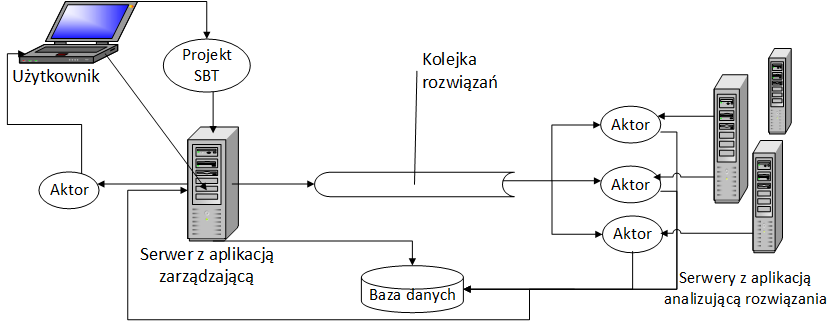
\includegraphics[width=1.05\hsize]{fig/scaxerciser_schemat}
\caption{Schemat komunikacji pomiędzy różnymi elementami systemu\label{system:schemat}}
\source{Opracowanie własne}
\end{figure}

Zanim jednak zostanie przedstawiona charakterystyka obu aplikacji i metod komunikacji między nimi, należy odpowiedzieć na pytanie czym są \emph{Akka} i aktorzy.

\subsection{Aktorzy}

Akka to zestaw narzędzi do tworzenia aplikacji działających na maszynie wirtualnej JVM, które potrafią obsługiwać wiele żądań równolegle, wchodzą w kontakt~z~klientem w sposób asynchroniczny i wspierają zdarzeniowy model programowania. W jej skład wchodzą specjalne komponenty -- aktorzy. Dają one szanse programistom w pełni skupić się na tym jak zaimplementować w aplikacji założone cele poprzez zdjęcie z nich odpowiedzialności za skalowalność kodu i zarządzanie zasobami.   

Moduły Akki to tak naprawdę pliki archiwów \emph{.jar}. Można z nich korzystać jak z każdej innej biblioteki w tej postaci. Zaletą każdego z komponentów jest to, że posiada zminimalizowaną listę zależności. Moduł aktorów nie wymaga niczego innego ponad standardową biblioteką Scali. W rzeczywistości od wersji 2.10 Scali moduł ten zawarty jest jako część standardowej biblioteki języka. 

Wykorzystanie aktorów ma na celu uruchamianie procesów działających równolegle i rozwiązujących wspólnie pewne zadania, komunikując się przy tym ze sobą~w~sposób asynchroniczny. Autorzy książki ,,Akka in Action'' \cite[s. 9]{Roestenburg:2012:AIA} jako przykład zastosowania aktorów podają system sprzedający bilety. Załóżmy, że istnieje jedna pula biletów na koncert oraz cztery kasy. Typowa implementacja takiego systemu w Akkce oparta będzie na aktorach komunikujących się ze sobą niemutowalnymi wiadomościami. Każdy z nich posiada informację o adresie innych aktorów. Pierwszym aktorem niech będzie dystrybutor biletów, a kolejnymi agenci odpowiadający za sprzedaż.

Dystrybutor posiada informację, że na dany koncert dostępnych jest na przykład 100 biletów. Najprostszym sposobem powiadomienia o tym agentów jest wysłanie tej informacji w sposób łańcuchowy. Aktor dystrybutora przesyła zatem tę wiadomość do pierwszego aktora kasy. Ten odejmuje z puli wszystkich biletów swoją część i przekazuje nową wiadomość do drugiego aktora kasy. Wiadomość ta również zawiera informacje o tym ile biletów zostało wziętych z puli oraz ile zostało. Sytuacja powtarza się, aż każda z kas będzie posiadać dokładnie 25 biletów.

Mocną stroną takiego rozwiązania jest to, że aktorzy kas mogą sprzedawać równolegle bilety bez blokowania siebie nawzajem. Każdy z nich posiada przecież własną pulę wejściówek. Innym plusem jest to, że aktorzy nie muszą czekać na odpowiedź dystrybutora. W sytuacji, gdy dystrybutor ulegnie awarii to kasy nadal mogą pracować aż do momentu wyprzedania puli biletów. Dodatkowo, gdy agent wyśle wiadomość do zepsutego dystrybutora to nie ulegnie on awarii, ani nie będzie czekać na odpowiedź. Jego praca nie zostanie przerwana, a jego żądanie może zostać obsłużone przez inny obiekt.

Podsumowując, aktorzy w powyższym przykładzie nie współdzielą danych,~a~komunikują się przez niemutowalne wiadomości. Unika się zatem problemów spotykanych w klasycznych wielowątkowych implementacjach. Są to blokady związane z dostępem do danych, czy zakleszczanie wątków\footnote{Sytuacja, w której co najmniej dwa różne wątki czekają na siebie wzajemnie.}. Akka wyklucza większość tego typu problemów uwalniając programistę od dodatkowego ciężaru.

Zaimplementowany w Scali system aktorów Akki dba o to, by poszczególni aktorzy potrafili komunikować się ze sobą oraz dostarcza wymagane komponenty do pracy z nimi. Możliwe jest korzystanie z niego także w programach Javowych. Akka dla Scali dostarcza cechę \texttt{Actor} na podstawie, której możliwe jest skonstruowanie własnego aktora. Stworzenie wspominanego agenta kasy ograniczyłoby się zatem do skonstruowania klasy rozszerzającej tę cechę i zawierającą liczbę wolnych biletów na dany koncert. Akka nie pozwoli jednak na powołanie go do życia przy użyciu konstruktora, ponieważ dałoby to bezpośredni dostęp do jego metod. To z kolei byłoby niezgodne z ideą równoległej pracy poprzez przesyłanie wiadomości. System aktorów sam tworzy referencje aktorów\footnote{W Scali jest to obiekt typu \texttt{ActorRef}}. Pozwala na ich podstawie zlokalizować żądanego aktora.

Aktora Akki najprościej jednak można scharakteryzować przez pryzmat czterech głównych operacji jakie wykonuje:

\begin{enumerate}
\item Tworzenie -- każdy aktor może tworzyć nowych aktorów. W systemie Akki istnieje więc aktor będący na szczycie w hierchii.
\item Wysyłanie -- model programowania przy użyciu aktorów polega na przesyłaniu między aktorami asynchronicznych wiadomości. 
\item Odbieranie -- aktor odbiera wiadomości, od których uzależnione jest jego ,,zachowanie''. Występuje tutaj mechanizm dopasowywania wzorca.
\item Kontrolowanie -- aktor może monitorować potomnych aktorów poprzez odbieranie wiadomości i reagować w ten sposób na ewentualne błędy, czy niepowodzenia operacji przez nich wykonywanych.
\end{enumerate}

Prosty przykład kodu uruchamiającego aktora oraz wysyłającego mu wiadomości znajduje się poniżej. Jest to wariacja przykładu z dopasowywaniem wzorca z pierwszego rozdziału \ref{patternMatching:example}.

\begin{minted}[]{scala}
import akka.actor.{Actor, ActorSystem, Props}
case class Cat(name: String)
case class Dog(name: String)
object AnimalActor {
  def props = Props(new AnimalActor)
}
class AnimalActor extends Actor {
  def receive = {
    case c: Cat => println("Meow!")
    case d: Dog => println("Woof!")
    case _ => println("Animal")
  }
}
scala> val system = ActorSystem("animals")
system: akka.actor.ActorSystem = akka://animals

scala> val actor = system.actorOf(AnimalActor.props)
actor: akka.actor.ActorRef = Actor[akka://animals/user/\$\#b359028552]

scala> actor ! Cat("Tom")
Meow!

scala> actor ! Dog("Reksio")
Woof!
\end{minted}

\subsection{Aplikacja zarządzająca}

Aplikacja ta zajmuje się wszystkimi operacjami związanymi z tworzeniem zadań, grup, czy zarządzaniem użytkownikami. Tym ostatnim udostępniony zostaje interfejs w postaci strony internetowej. Jej poszczególne elementy są wyświetlane lub ukrywane w zależności od roli osoby aktualnie korzystającej z aplikacji. Każda ścieżka adresu prowadząca do widoku jest dodatkowo zabezpieczona. To znaczy, że nawet jeśli użytkownik odgadłby URL, pod którym znajduje się formularz dodawania grupy, a nie posiadałby odpowiednich uprawnień to zostanie mu wyświetlony widok błędu z odpowiednim komunikatem. 
Aplikacja składa się w rzeczywistości jedynie z dwóch stron - strony logowania oraz strony właściwej interfejsu. Dlatego też wyświetlenie tego komunikatu nie byłoby klasycznym przekierowaniem URL.
Panele dostępne użytkownikowi generowane są dynamicznie, a potrzebne dane pobierane od serwera w sposób asynchroniczny. Poza stroną logowania całość zbudowana została w oparciu o narzędzie \emph{AngularJS}, który umożliwia w szybki sposób osiągnąć taki efekt.

Aby w pełni zrozumieć komunikację przedstawioną na rysunku \ref{system:schemat} w tej części systemu należy poczynić najpierw kilka założeń. Załóżmy, że w systemie funkcjonują już grupy, które posiadają aktywne zadania stworzone przez prowadzących. 

Uczestnik loguje się do systemu by rozwiązać zadanie z wybranej grupy. W tym momencie \emph{WebSocket} zostaje powiązany z jego identyfikatorem poprzez żądanie \emph{Ajax} zrealizowane przez napisany dla \emph{AngularJS} serwis. Po stronie serwera zostaje wysłana wiadomość do aktora, który zajmować się będzie wiązaniem WebSocketów z identyfikatorami użytkownika. Następnie do przeglądarki zostaje wysłana odpowiedź ze statusem HTTP \texttt{OK}. Głównym zadaniem uruchomionego aktora jest powiadamianie później użytkownika o skończonej analizie jego rozwiązania. Reaguje on zatem na jeszcze dwie inne wiadomości -- zamykającą dwukierunkowe połączenie oraz zlecenie poinformowania użytkownika. Zaimplementowane rozwiązanie posiada tę zaletę, że jeśli użytkownik posiada więcej niż jedno okno otwarte, to wszystkie otrzymają tę samą informację. 

Po zapoznaniu się z opisem zadania i poleceniami do wykonania, użytkownik pobiera projekt SBT na swój dysk. Chcąc wysłać swoje rozwiązanie wykonuje polecenie \texttt{sendSolution} z poziomu projektu. Zostaje wówczas wysłane żądanie do aplikacji zarządzającej, która zweryfikuje dane użytkownika oraz zidentyfikuje zadanie, do którego odnosi się przesłane rozwiązanie. Gdy wszystkie wymagania zostaną spełnione, utworzony zostanie nowy wpis w bazie danych. Następnie identyfikator rozwiązania zostanie umieszczony w kolejce rozwiązań. Jest to server \emph{RabbitMQ}\footnote{\url{http://www.rabbitmq.com/}}, dzięki któremu obie aplikacje w sposób asynchroniczny mogą współpracować ze sobą.
  
Do ukończenia procesu weryfikacji pozostaje już tylko powiadomienie odpowiedniego użytkownika. Może to zrobić odbierając od aplikacji testującej żądanie HTTP po skończonej analizie. W ten sposób aktor zarządzający połączeniami WebSockets otrzyma wiadomość \texttt{Notify} zawierającą obiekt rozwiązania. Na podstawie umieszczonego w nim identyfikatora użytkownika serwer wyśle informację do właściwego klienta o skończonej operacji. Oczywiście jest to możliwe jeśli wcześniej aktor nie otrzymał wiadomości \texttt{SocketClosed} usuwającej z pamięci powiązanie z WebSocketem. Zamierzonym końcowym efektem jest jednak wyświetlenie użytkownikowi stosownego komunikatu oraz umieszczenie informacji o ocenie na liście ostatnio oddanych rozwiązań. 

\subsection{Aplikacja testująca kod}
 
Każda instancja aplikacji sprawdzającej kod startując uruchamia dowolną liczbę aktorów. Liczba aktorów jest zdefiniowana w pliku konfiguracyjnym podobnie jak ustawienia dotyczące połączenia z serwerem RabbitMQ. Uruchomiony aktor staje się odbiorcą odpowiadających za ściąganie wiadomości z kolejki rozwiązań. 

Powodem takiej implementacji jest potrzeba uniknięcia natychmiastowego testowania rozwiązań. Operacja taka może zająć zbyt dużą ilość czasu, aby oczekiwać wyniku przez zwykłe żądanie HTTP. Dodatkowym problemem są również ograniczone zasoby serwerów. Jednoczesne sprawdzanie ogromnej ilości rozwiązań może doprowadzić do błędów z tym związanych. Zamiast tego możliwe jest ustalenie ile rozwiązań ma być testowanych jednocześnie. Pozostałe będą oczekiwać w kolejce i zostaną sprawdzone, gdy tylko będzie to możliwe. RabbitMQ domyślnie wysyła do swoich odbiorców wiadomości, gdy tylko są w stanie gotowości.

System został tak skonfigurowany, aby w przypadku, gdy jeden z aktorów ulegnie awarii lub zostanie wyłączony w trakcie przetwarzania wiadomości z kolejki to nie zostaną utracone żadne dane. RabbitMQ oczekuje potwierdzenia wykonania od swoich odbiorców. Jeśli utraci z którymś kontakt to wiadomość zostanie zinterpretowana jako nie przetworzona i przesłana do innego aktora. Przewidziana została także sytuacja, w której awarii może ulec serwer RabbitMQ. Kolejka~i~wiadomości przesyłane do niej posiadają ustawienia, które w takim przypadku zostaną zapisane na dysku. Uruchomiony ponownie serwer odczyta je. 

Po odebraniu wiadomości z kolejki zostaje uruchomiony proces odbudowy projektu SBT i testowania. Każde rozwiązanie jest sprawdzane w osobnym i tymczasowym katalogu. Pobrane z bazy danych zostają wgrane przez prowadzącego grupę pliki z testami oraz projektem dla sprawdzanego zadania. Oczywiście w bazie danych znajdują się także zmodyfikowane przez uczestnika pliki i one również zostają odzyskane. Wszystkie te elementy odpowiednio połączone ze sobą stworzą nowy projekt SBT. 

ScalaTest pozwala na uruchamianie testów w projekcie przy pomocy tak zwanego \emph{reportera}. Jest to specjalny obiekt przechwytujący szczegółowe informacje~o~testach. Napisany na potrzeby systemu reporter reaguje na zdarzenia wyzwalane przez ScalaTest i zapisuje dane do pliku \emph{.json}. 

Gdy proces testowania zostanie zakończony następuje odczytanie wyników~i~odzwierciedlenie ich w postaci obiektu typu \texttt{Result}. Klasa \texttt{Result} zawiera pola informujące między innymi o liczbie spodziewanych, ukończonych, anulowanych, czy wszystkich testów. Dopełnieniem jest pole \texttt{mark}, z którego odczytać można jaki procent testów zakończonych zostało sukcesem w stosunku do liczby wszystkich testów w projekcie. 

Wpis o danym rozwiązaniu zostaje zmodyfikowany w bazie danych o zwrócone przez reportera szczegóły. Dodatkowo, informacja o rozwiązaniu jest uzupełniona o domyślny raport końcowy zwracany przez ScalaTest, a także o szczegóły uruchomionego przez aplikację procesu. Ostatnim krokiem jest powiadomienie aplikacji zarządzającej o zakończonej analizie wysyłając żądanie HTTP. Aktor staje się gotowy do odebrania kolejnej wiadomości z kolejki po wykonaniu wszystkich opisanych wyżej akcji.

\section{Zastosowane technologie}

Na ostateczny kształ systemu miało wpływ wiele technologii. Część z nich została już opisana w poprzednich rozdziałach. Są to między innymi SBT, ScalaTest, ScalaCheck, czy AKKA. Warto jednak przyjrzeć się po krótce w jaki sposób zaimplementowana zostały pozostałe elementy systemu. 

Pierwszy przedstawiony zostanie \emph{Play Framework}. To właśnie przy jego pomocy powstały dwie aplikacje, na które składa się całość systemu. Narzędzie to pozwala stworzyć aplikację internetową w oparciu o wzorzec Model-Widok-Kontroler w języku Java lub Scala. Składa się między innymi z wydajnego serwera HTTP i kompilatora. Zmiany wprowadzane do aplikacji mogą być widoczne bez potrzeby przebudowania całego projektu. Aplikacja bowiem jest automatycznie rekompilowana w trakcie działania. Play wspiera podejście REST oraz posiada zintegrowaną bazę danych\footnote{Domyślnie jest to H2}. Bez przeszkód można jednak połączyć się z innymi bazami. 

System weryfikacji kodu musi przechowywać, gdzieś pliki projektów i testów. \emph{MongoDB} to nierelacyjna baza danych z mechanizmem gotowym do przechowywania plików o rozmiarach przekraczajacych nawet 16 MB. Wszystkie oficjalne sterowniki tej bazy danych wspierają ten mechanizm, w tym oczywiście również dla Scali. Ponadto do pobierania statystyk grupy wykorzystana została technika agregacji. To znaczy, że kolejne instrukcje bazy danych są wykonywane łańcuchowo w oparciu o kolejne wyniki poprzednich operacji.

RabbitMQ oraz jego zastosowanie w systemie zostało w skrócie przedstawione w podrozdziale \ref{section:struktrura}. Warto jednak przyjrzeć się temu narzędziu jeszcze bliżej. W tym rozdziale zostanie przedstawione w jaki sposób skonfigurować połączenie z nim od strony aplikacji. Ponieważ aplikacje korzystają z oficjalnego klienta tego serwera dla Javy, będzie to także kolejny dowód na kompatybilność Scali.

Na zakończenie omówiony zostanie interfejs użytkownika, który niemal w całości powstał przy użyciu biblioteki języka JavaScript - \emph{AngularJS}. Ona również korzysta z wzorca Model-Widok-Kontroler. To właśnie wiązanie tych trzech warstw jest szczególnie mocną stroną AngularJS. Dodatkowo posiada własny kompilator HTML, który okazał się niezwykle pomocny w ukrywaniu elementów strony przed nieautoryzowanym użytkownikiem.  

\subsection{Play Framework}

Play Framework można w pewnym sensie porównać do \emph{Ruby on Rails}. Oba te narzędzia korzystając z archtektury Model-Widok-Kontroler dostarczają szkielet aplikacji internetowych, które sprawdzają się doskonale w małych i średnich projektach. W obu przypadkach mamy również do czynienia ze wsparciem wzorca REST. To znaczy, że klient i serwer komunikują się ze sobą w oparciu o \emph{zasoby} (ang: resources). Adres URL powinien wtedy zawierać parametry w ścieżce identyfikującej dany zasób lub zasoby. Wykorzystane ku temu zostają cztery metody HTTP:

\begin{itemize}
\item GET -- pobranie zasobu lub zasobów
\item POST -- wprowadzenie nowych danych
\item PUT\footnote{Od wersji 4.0 Ruby on Rails zalecane jest korzystanie z metody PATCH} -- edytowanie zasobu
\item DELETE -- usunięcie danych
\end{itemize}

Właśnie takie rozwiązanie jest zaimplementowane przede wszystkim w aplikacji zarządzającej. Zasobami są w niej użytkownicy, grupy, zadania oraz rozwiązania. Podobieństw do idei proponowanej przez Ruby on Rails jest więcej. Wszelkie ustawienia aplikacji umieszczone są w specjalnych plikach konfiguracyjnych. Biblioteki, zależności projektu ściągane są automatycznie przez narzędzie po umieszczeniu odpowiednich linii w pliku do tego przeznaczonym. Samo wygenerowanie szkieletu sprowadza się do wpisania jednego polecenia \texttt{play new nazwaAplikacji} podczas, gdy w Ruby on Rails jest to \texttt{rails new nazwaAplikacji}.

Aplikacje powstałe z Play Framework pracują bezstanowo. Oznacza to, że nie jest przechowywana na serwerze sesja powiązana z danym użytkownikiem. Zamiast tego zalecane jest trzymanie wielu informacji po stronie klienta lub zapisywanie sesji w bazie danych. Play wspiera również technikę rozproszonej pamięci podręcznej po stronie serwera. Twórcy twierdzą, że w ten sposób aplikacje powstałe przy użyciu ich narzędzia są dużo bardziej skalowalne.

Play zawiera zintegrowany kompilator Javy i Scali. Podczas tworzenia aplikacji możliwe jest uruchomienie jej w środowisku deweloperskim i utrzymywanie ją w stanie działania. Wszystkie wprowadzane do kodu zmiany będą na bieżąco aktualizowane i widoczne. Jest to zdecydowana oszczędność czasu, gdyż nie ma potrzeby przebudowywania aplikacji i uruchamiania ponownie serwera. 

Zasobami udostępnianymi przez aplikację są oczywiście modele. W wersji dla Scali odwzorowuje je się przy pomocy \texttt{case class} oraz \texttt{object}. Wszystkie ich atrybuty są trzymane w postaci pól klas. Natomiast logika biznesowa powinna być zaimplementowana w postaci metod singletonu o tej samej nazwie co encja. Jest to ,,obiekt towarzyszący'' (ang: companion object) zdefiniowany w tym samym pliku. Posiada on również dostęp do pól prywatnych w danych klasach. Prosty przykład modelu znajduje się poniżej. Klasa \texttt{Cat} posiada obiekt towarzyszący o tej samej nazwie. Zawarta w nim metoda \texttt{meowAndName} jako parametr bierze obiekt typu \texttt{Cat}. Zwraca ciąg znaków składający się z wartości pola \texttt{name} z podanego argumentu.

\begin{minted}[fontsize=\small]{scala}
package models

case class Cat(name: String)

object Cat {
  def meowAndName(cat: Cat): String = "Meow! " + cat.name
}

scala> Cat.meowAndName(Cat("Nazir"))
res0: String = Meow! Nazir
\end{minted}

Warto też dodać, że Play Framework posiada wtyczki do popularnych zintegrowanych środowisk programistycznych jak IntelliJ IDEA, czy eclipse. Obie aplikacje i szablon projektu SBT udostępniany przez część zarządzającą systemu mają dołączone zależności pozwalające wygenerować potrzebne pliki do zaimportowania projektu do tych narzędzi. W ten sposób praca z Play Framework staje na równi z innymi już dojrzałymi narzędziami. Zyskuje się bowiem wparcie w postaci łatwego uruchamiania aplikacji, czy rozpoznawania składni plików specyficznych dla Play.

\subsection{MongoDB}

MongoDB to wydajna baza przechowująca dane w postaci dokumentów. Jeden serwer MongoDB może się składać z wielu baz danych. Pojedyńcza baza danych zawiera z kolei kolekcje, które są zbiorem wspomnianych dokumentów. Ściślej mówiąc są to obiekty w postaci notacji \emph{JSON}. Dokumenty mogą być dynamicznie modyfikowane i nie są ograniczone przez żaden schemat nakładany na kolekcje. Oznacza to w praktyce, że dokumenty w obrębie kolekcji mogą mieć różny zestaw pól.

Zasiegając informacji z oficjalnej strony\footnote{\url{http://www.mongodb.org/}} można scharakteryzować MongoDB w kilku punktach:

\begin{itemize}
\item elastyczność -- przechowywanie danych w postaci obiektów JSON i brak ograniczeń ze strony schematów nakładanych na kolekcje ułatwia modyfikację modelu danych wraz z ewolucją projektu.
\item możliwości utrzymaniowe -- dostarczenie cech takich jak dodatkowe indeksy, łańcuchowe wykonywanie zapytań, czy bogate instrukcje aktualizacji. Wśród nich taka, która w przypadku nie odnalezienia dokumentu dokumentu przez zapytanie potrafi stworzyć nowy wpis w bazie. W skład MongoDB wchodzi \emph{Aggregation Framework}, którego głównym zadaniem jest obliczanie różnych wartości na podstawie przechowywanych danych.
\item szybkość -- jest to nierelacyjna baza danych. Dokumenty wiąże się ze sobą przeważnie poprzez tak zwane zagnieżdzone kolekcje. Sprawia to, że wyszukiwanie danych jest szybsze niż w relacyjnej bazie składającej się z wielu tabel. Nie jest konieczne bowiem łączenie tabel ze sobą na potrzeby niektórych zapytań.
\item łatwa w użyciu - MongoDB jest łatwa w instalacji i konfiguracji. Instalacja sprowadza się do wykonania zaledwie kilku kroków, po zakończeniu których baza jest gotowa do użycia. Programista może skupić się na rozwijaniu swojej aplikacji zamiast spędzać czas nad skomplikowaną konfiguracją.
\end{itemize}

Oficjalny sterownik dla języka Scala nosi nazwę \emph{Casbah}. Jest to tak naprawdę ,,opakowanie'' sterownika dla Javy. Społeczność Scali wytworzyła również wiele dodatkowych narzędzi do współpracy z tą bazą danych. Najpopularniejszy z nich do \emph{Salat}. System weryfikacji kodu Scala korzysta z obydwu.

MongoDB udostępnia powłokę, w której można wykonywać zapytania posługując się składnią JavaScriptu. Podejście prezentowane przez Casbah polega na odzwierciedleniu składni tych zapytań w języku Scala.  
Przykładowo chcąc w systemie znaleźć rozwiązania ocenione na co najmniej 80 procent należy zrealizować poniższe zapytanie w powłoce MongoDB:

\inputminted[fontsize=\small]{javascript}{code/mongoFind.js}

Casbah dostarcza specjalny typ \texttt{MongoDBObject}. Dzięki nim można zbudować bardzo podobne instrukcje. Obiekty tego typu są podawane jako argumenty metod o tych samych nazwach. Są to \texttt{find}, \texttt{findOne}, \texttt{update}, \texttt{count} i wiele innych. Po skonfigurowaniu połączenia z bazą i stworzeniem instancji odpowiadającej za kolekcję w bazie danych możliwe jest wykonanie zapytania w poniższej formie:

\inputminted[fontsize=\small]{scala}{code/casbahFind.scala} 

Nie jest to jednak zbyt czytelne rozwiązanie. Szczególnie, gdy pobierane dane filtrowane są przez wiele warunków. Niestety metody dostaczane przez Salat w dużej części jako argumenty również przyjmują \texttt{MongoDBObject}. Nieco lepiej wygląda sytuacja, gdy aktualizowany lub tworzony jest dany obiekt. Wtedy argumentem staje się odpowednik dokumentu w Scali reprezentowany przez klasę.

Salat skupia się na obiekcie towarzyszącym. Musi on rozszerzać cechę \texttt{ModelCompanion}. W zamian narzędzie dostarcza:

\begin{itemize}
\item metody do konwersji obiektów z i do formatu JSON
\item zestaw metod aktualizujących, zapisujących i usuwających obiekty z bazy danych
\item gotowe metody do wyszukiwania tylko po identyfikatorze
\item pozostałe metody wykonujące zapytania jak \texttt{find}, czy \texttt{count}
\end{itemize}

Na zakończenie należy odnieść się do wspominanego mechanizmu przechowującego pliki -- \emph{GridFS}. Pliki wgrywane do bazy przy użyciu tej techniki są dzielone na mniejsze kawałki i przechowywane w bazie jako osobne dokumenty. Po dodaniu pierwszego pliku utworzone zawsze zostają dwie kolekcje. Jedna z nich przechowuje dokumenty-kawałki pliku, a druga ogólne informacje o pliku. Są to to między innymi nazwa, rozmiar pliku, czy jego typ. Sterownik automatycznie potrafi odnaleźć potrzebne kawałki i połączyć je ze sobą, gdy wykonane jest zapytanie. 

\subsection{RabbitMQ}

Kolejkowanie rozwiązań pomiędzy dwoma aplikacjami nie byłoby możliwe bez technologii opartej na protokole AMQP\footnote{AMQP - jest to skrót od Advanced Message Queuing Protocol}. Jest to protokół w warstwie aplikacji służący do przesyłania asynchronicznych wiadomości. Pracując na tym protokole mamy do czynienia z dwoma bytami -- nadawcami i odbiorcami. Jak nie trudno się domyślić nadawca odpowiada za wysłanie wiadomości, natomiast odbiorca zbiera je i wykonuje operację często pochłaniającą większą ilość czasu. Zadaniem RabbitMQ jest rozdzielanie wiadomości pomiędzy właściwymi odbiorcami. W systemie weryfikacji kodu Scala czyni to właśnie za pomocą kolejki.

Konfiguracja kolejki w systemie jest bardzo prosta. Ustawienia mogą być różne w zależności od środowiska uruchomieniowego aplikacji. Odpowiadają za to oddzielne pliki.

\begin{itemize}
\item application.conf -- najbardziej ogólne ustawienia. Będą stosowane we wszystkich środowiskach.
\item application.dev.conf -- ustawienia środowiska deweloperskiego.
\item application.prod.conf -- ustawienia środowiska produkcyjnego.
\item application.test.conf -- ustawienia środowiska testowego.
\end{itemize} 

W aplikacji zarządzającej są to dwa ustawienia definiujące host, na którym działa RabbitMQ oraz nazwę kolejki rozwiązań.

\begin{alltt}
rabbitmq.host=localhost
rabbitmq.solutions.queue=solutions_queue
\end{alltt}

Aplikacja testująca kod posiada dodatkowe pole konfiguracyjne określające ilość uruchamianych aktorów analizujących rozwiązania.

\begin{alltt}
rabbitmq.solutions.analyzers.number=2
\end{alltt}

W obu przypadkach ustawienia są wczytywane przy starcie aplikacji i zapisywane jako stałe pola obiektu \texttt{MQConfig}. Za wysłanie wiadomości do kolejki odpowiada metoda \texttt{send} obiektu \texttt{SolutionSender}.

\begin{minted}[]{scala}
private def send(solutionId: String) {
  val sendingChannel = RabbitMQConnection.connection.createChannel()
  sendingChannel.queueDeclare(MQConfig.RabbitMQSolutionsToAnalyzeQueue, 
    queueDurable, false, false, null)
  sendingChannel.basicPublish("", MQConfig.RabbitMQSolutionsToAnalyzeQueue, 
    MessageProperties.PERSISTENT_TEXT_PLAIN, solutionId.getBytes)
  sendingChannel.close()
}
\end{minted}

\texttt{RabbitMQConnection} to obiekt, którego zadaniem jest zarządzanie połączeniem z RabbitMQ zdefiniowanego w pliku konfiguracyjnym. By wysłać wiadomość potrzebne jest utworzenie na nim kanału i zadeklarowanie kolejki. W rozdziale \ref{section:struktrura} powiedziane zostało, że wiadomości wrzucone do kolejki są zabezpieczone przed utratą w przypadku awarii serwera. Między innymi w metodzie \texttt{queueDeclare} odpowiada za to zmienna logiczna \texttt{ququeDurable}. Ustawiona wartość na \texttt{true} oznacza, że RabbitMQ będzie pamiętać o tej kolejce przy ponownym uruchomieniu. W metodzie wysyłającej wiadomość -- \texttt{basicPublish} -- drugim argumentem jest ustawienie pochodzące z klienta RabbitMQ. Gwarantuje ono zapamiętanie wiadomości wysyłanej do kolejki.

W aplikacji testującej zbieranie wiadomości z kolejki odbywa się przez metodę \texttt{startRecevingMessages} wywołanej po wysłaniu polecenia startowego do aktora.

\begin{minted}[]{scala}
def startRecevingMessages() {
  val queueDurable = true
  val prefetchCount = 1
  val autoAck = false
  channel.queueDeclare(queueName, queueDurable, false, false, null)
  channel.basicQos(prefetchCount)
  val consumer = new QueueingConsumer(channel)
  channel.basicConsume(queueName, autoAck, consumer)
  while (true) {
    val delivery = consumer.nextDelivery()
    val solutionId = new String(delivery.getBody)
    ...
    channel.basicAck(delivery.getEnvelope.getDeliveryTag, false)
  }
}
\end{minted}

W tym przypadku mamy również do czynienia z deklaracją kolejki oraz kanałem transmisji. Odbieranie wiadomości z przez odbiorcę RabbitMQ wykonywane jest w nieskończonej pętli. To co przede wszystkim ma pokazać powyższy przykład to zmienna \texttt{autoAck} przekazana jako drugi argument metody \texttt{basicConsume}. Ustawiona na wartość logiczną \texttt{false} sprawia, że RabbitMQ będzie oczekiwać od odbiorcy potwierdzenia wykonania zadania. Jeśli odbiorca ulegnie awarii to RabbitMQ zinterpretuje wiadomość, którą otrzymał jako nie przetworzoną i przekaże ją do innego odbiorcy.

Dzięki kompatybilności Scali oraz oficjalnemu klientowi RabbitMQ dla języka Java mamy w powyższych przykładach w rzeczywistości do czynienia z wywołaniami metod Javovych.

\subsection{AngularJS}

Interfejs aplikacji zarządzającej składa się jedynie z dwóch stron. Pierwsza z nich to strona logowania. Zbudowana została przy pomocy metod dostarczanych przez Play Framework do tworzenia formularzy w widokach. Użytkownik po zalogowaniu zostaje przekierowany na stronę główną, gdzie dołączone są pliki ze skryptami JavaScript. Wśród nich znajduje się AngularJS i logika interfejsu działająca przy jego użyciu.

AngularJS to wyprodukowane i wspierane przez Google narzędzie. Ideą było stworzenie instrumentu, który pozwoliłby na szybkie budowanie małych i dynamicznych aplikacji internetowych. Inżynierom Google'a cel udało się osiągnąć poprzez wprowadzenie własnego kompilatora HTML oraz podwójnego wiązania danych.

Kompilator HTML pozwala programiście zdefiniować kod strony w zupełnie nowy sposób. Istnieje możliwość tworzenia własnych znaczników, czy atrybutów. W ten sposób można dodać specyficzne dla potrzeb aplikacji ,,zachowanie'' poszczególnych elementów strony. Programista dokonuje tego poprzez napisanie własnych dyrektyw. Część zarządzająca omawianego systemu potrzebowała dyrektyw decydujących o tym, które z elementów strony powinny być widoczne, bądź ukryte w zależności od roli zalogowanego użytkownika. Dzięki kompilatorowi udało się stworzyć czytelne dla każdego atrybuty HTML.

\begin{minted}[]{html}
<div has-permission="Educator" class="pull-right">
...
</div>
\end{minted}

Fragment strony zawarty pomiędzy znacznikami \texttt{div} w powyższym przykładzie będzie pokazany jedynie prowadzącemu. Jego rola w kodzie systemu określona jest jako \texttt{Educator} (ang: dydaktyk). Stworzona dyrektywa pozwala zdefiniować wyświetlaną zawartość dzięki dodaniu czytelnego atrybutu \texttt{has-permission}.

Podwójne wiązanie danych w sposób automatyczny synchronizuje to co jest wyświetlane na stronie, z tym co znajduje się w kontrolerze JavaScript odpowiadającym za konkretny widok. Kompilator AngularJS prezentuje ,,na żywo'' wyniki kolejnych etapów kompilacji. Wszelkie zmiany w widoku są odzwierciedlone w modelu danych i odwrotnie. Chociaż kontroler jest osobnym bytem to możliwe jest modyfikowanie w nim danych bez potrzeby samodzielnego manipulowania elementami strony.  

Obiekt, który zajmuje się wiązaniem modelu z widokiem to \texttt{\$scope}. Jest wstrzykiwany do funkcji kontrolera na etapie kompilacji. Poniżej znajduje się fragment kontrolera odpowiadającego za widok listy zadań w danej grupie.

\inputminted[fontsize=\small]{javascript}{code/angularController.js} 

W ciele funkcji do obiektu \texttt{\$scope} dodany zostaje atrybut \texttt{group}. Jego wartością jest grupa zwracana przez serwer w postaci JSON. Za wysyłanie właściwych żadań do serwera odpowiadają serwisy. W tym wypadku jest to \texttt{Group}, który posiada metodę \texttt{show}. Przyjmuje ona jako argument również obiekt. Wewnątrz metody, atrybut \texttt{id} zostaje dołączony przez AngularJS do adresu URL prowadzącego do danego zasobu.

Podwójny nawias klamrowy pozwala korzystać z dodanych do \texttt{\$scope} obiektów w kodzie HTML. 

\begin{minted}[]{html}
<div class="panel-heading">
 Szczegóły zadania: {{assignment.title}}, z grupy: {{group.name}}
 ...
</div>
\end{minted}

Do \texttt{\$scope} można dodać również funkcję. Następnie korzystając z dostarczanych domyślnie przez AngularJS dyrektyw, wywoływać ją na stronie. Jedną z nich może być na przykład \texttt{ng-click}. Prowadzi to do lepszej organizacji kodu w aplikacji. Funkcje wykonujące specyficzne operacje dla widoku zdefiniowane są bowiem w odpowiadającym mu kontrolerze. 

AngularJS sprawia, że aplikacja internetowa zbudowana jest z dostarczanych przez narzędzie modułów. Nie trzeba znać ich wszystkich, aby stworzyć dynamiczny interfejs. W miarę rozwoju projektu odkrywane są, bowiem nowe funkcjonalności. Programiści wdrażają je komponując kolejne moduły (serwisy, kontrolery) specyficzne dla danej aplikacji.  

% zakończenie 
\summary
Scala to język warty szczególnej uwagi. Łączenie ze sobą paradygmatu programowania obiektowego i funkcyjnego oraz kompatybilność z JVM stwarza ogromne możliwości. W wielu miejscach już teraz mogłaby swobodnie zastąpić Javę. System weryfikacji jakości kodu Scala pozwala przy użyciu dojrzałych narzędzi testowania nie tylko zweryfikować kod, ale również przyczynić się do wzrostu popularności języka. Zawiera w sobie element dydaktyczny, pozwalający na definiowanie własnych kursów i zadań. Implementując go w ośrodkach edukacyjnych, ma szansę przyczynić się do wzrostu zainteresowania programowaniem i podniesieniem umiejętności przyszłych programistów. Z powodzeniem mógłby być również wykorzystywany w firmach chcących, sprawdzić kwalifikacje kandydatów w procesie rekrutacyjnym.
System powstał przy użyciu wielu nowoczesnych technologii i jest dostosowany do pracy w architekturze rozproszonej.

% załączniki (opcjonalnie):
%\appendix
%\chapter{Tytuł załącznika jeden}

%Treść załącznika jeden.

%\chapter{Tytuł załącznika dwa}

%Treść załącznika dwa.

% wymuszenie pokazania bibliografii
%\nocite{Hinojosa:2013:TIA}

% literatura (obowiązkowo):
\bibliographystyle{unsrt}
\bibliography{xml}

% spis tabel (jeżeli jest potrzebny):
\listoftables

% spis rysunków (jeżeli jest potrzebny):
\listoffigures

\oswiadczenie

\end{document}
